\documentclass{article}
\usepackage[a4paper, margin=3mm, landscape]{geometry}
\usepackage{multicol}
\usepackage{xcolor}
\usepackage{enumitem}
\usepackage{amsmath}
\usepackage{amsfonts}
\usepackage{listings}
\usepackage{soul}
\usepackage{graphicx}

\pdfinfo{
    /Title (CS2109S.pdf)
    /Creator (TeX)
    /Producer (pdfTeX 1.40.0)
    /Author (Jason Qiu)
    /Subject (CS2109S)
    /Keywords (CS2109S, nus, cheatsheet, pdf)
}

\graphicspath{ {./img/} }

\pagestyle{empty}
\setcounter{secnumdepth}{0}
\setlength{\columnseprule}{0.25pt}

% Redefine section commands to use less space
\makeatletter
\renewcommand{\section}{\@startsection{section}{1}{0mm}%
    {-1ex plus -.5ex minus -.2ex}%
    {0.5ex plus .2ex}%x
{\normalfont\large\bfseries}}
\renewcommand{\subsection}{\@startsection{subsection}{2}{0mm}%
    {-1explus -.5ex minus -.2ex}%
    {0.5ex plus .2ex}%
{\normalfont\normalsize\bfseries}}
\renewcommand{\subsubsection}{\@startsection{subsubsection}{3}{0mm}%
    {-1ex plus -.5ex minus -.2ex}%
    {1ex plus .2ex}%
{\normalfont\small\bfseries}}%
\makeatother

% Adjust spacing for all itemize/enumerate
\setlength{\leftmargini}{0.5cm}
\setlength{\leftmarginii}{0.5cm}
\setlist[itemize,1]{leftmargin=2mm,labelindent=1mm,labelsep=1mm}
\setlist[itemize,2]{leftmargin=2mm,labelindent=1mm,labelsep=1mm,label=$\bullet$}

% Font
\renewcommand{\familydefault}{\sfdefault}

% Define colors for math formulas
\definecolor{myblue}{cmyk}{1,.72,0,.38}
\everymath\expandafter{\the\everymath \color{myblue}}

% Custom command for keywords
\definecolor{highlight}{RGB}{251,243,218}
\newcommand{\keyword}[2][]{\sethlcolor{highlight}\hl{\textbf{#2}} #1 - }
\newcommand{\ilkeyword}[1]{\sethlcolor{highlight}\hl{\textbf{#1}}}

% Define colors and style for code
\definecolor{codegreen}{rgb}{0,0.6,0}
\definecolor{codegray}{rgb}{0.5,0.5,0.5}
\definecolor{codered}{HTML}{CC241D}
\definecolor{backcolor}{rgb}{0.95,0.95,0.95}
\lstdefinestyle{codestyle}{
    backgroundcolor = \color{backcolor},
    commentstyle = \color{codegray},
    keywordstyle = \color{codered},
    stringstyle = \color{codegreen},
    basicstyle = \ttfamily,
    breakatwhitespace = false,
    showstringspaces = false,
    breaklines = true,
    showtabs = false,
    tabsize = 2
}
\lstset{style = codestyle}

% -----------------------------------------------------------------------
\begin{document}
\begin{multicols*}{3}
\footnotesize

% Title box
\begin{center}
    \fbox{
        \parbox{0.8\linewidth}{
            \centering \textcolor{black}{
                {\Large\textbf{CS2109S}} \\
                \normalsize{AY22/23 Sem 2}} \\
                {\footnotesize \textcolor{gray}{github.com/jasonqiu212}}
        }
    }
\end{center}

\section{01. Introduction}

\begin{itemize}
    \item \keyword{Agent}{Anything that can perceive its environment through sensors and acting upon that env. through actuators}
    \item \keyword{Agent Function}{Maps from percept histories to actions}
    \item \keyword{Rational Agent}{Chooses an action that is expected to maximize its performance measure, given by percept sequence and built-in knowledge}
    \item \keyword{Autonomous Agent}{If behavior is determined by its own expereince}
\end{itemize}

\subsection{Performance Measure of Function}

\begin{itemize}
    \item Motivation: For an agent to do the right thing, need a measure of goodness
\end{itemize}

\subsection{Defining the Problem: PEAS}

\begin{enumerate}
    \item Performance measure
    \item Environment
    \item Actuators
    \item Sensors
\end{enumerate}

\subsection{Characterizing the Environment}

\begin{enumerate}
    \item \keyword{Fully observable}{(vs. Partially) Agent's sensors can access complete state of env. all the time}
    \item \keyword{Deterministic}{(vs. Stochastic) Next state of env. is determined by \textbf{current state} and \textbf{action executed by agent}}
    \begin{itemize}
        \item \keyword{Strategic}{If env. is deterministic except for actions of other agents}
    \end{itemize}
    \item \keyword{Episodic}{(vs. Sequential) Agent's experience is divided into atomic \textbf{episodes}, where each episode includes perceiving and an action, and \textbf{action depends on episode} itself}
    \item \keyword{Static}{(vs. Dynamic) Env. is unchanged while agent is deciding}
    \begin{itemize}
        \item \keyword{Semi}{Time does not affect env., but affects performance score}
    \end{itemize}
    \item \keyword{Discrete}{(vs. Continuous) Discrete num. of percepts and actions}
    \item \keyword{Single Agent}{(vs. Multi-agent) Agent operating by itself in an env.}
\end{enumerate}

\subsection{Implementing Agents (in ascending complexity)}

\begin{enumerate}
    \item \keyword{Simple Reflex Agents}{Fixed conditional rules}
    \item \keyword{Model-based Reflex Agents}{Stores percept history to make decisions about internal model of world with conditional rules. Eg. Roomba}
    \item \keyword{Goal-based Agents}{Keep in mind a goal and action aims to achieve it}
    \item \keyword{Utility-based Agents}{Find best way to achieve goal}
    \item \keyword{Learning Agents}{Learn from previous experiences}
\end{enumerate}

\subsection{Exploitation vs. Exploration}

\begin{itemize}
    \item \keyword{Exploitation}{Maximize expected utility using current knowledge of world}
    \item \keyword{Exploration}{Learn more about the world to improve future gains. May not always maximize performance measure.}
\end{itemize}

\section{02. Uninformed Search}

\begin{itemize}
    \item Deterministic, fully observable
    \item \keyword{Tree Search}{Can revisit nodes}
    \item \keyword{Graph Search}{Tracks visited (Tree Search + Memoization)}
    \item \keyword{Uninformed Search}{Uses only information available in problem definition}
\end{itemize}

\subsection{Formulating the Problem}

\begin{enumerate}
    \item How to represent state in problem?
    \item Initial state
    \item Actions: Successor function
    \item Goal test
    \item Path cost
\end{enumerate}

\begin{itemize}
    \item \keyword{Abstraction Function}{Maps abstracted representation to real world state}
    \item \keyword{Representation Invariant}{$I(c) = \textbf{True} \rightarrow \exists a \textbf{ s.t. } AF(c) = a$}
\end{itemize}

\subsection{Breadth-first Search}

\begin{itemize}
    \item Idea: Expand shallowest unexpanded node using \textbf{queue}
    \item Given: $b$: Branching factor and $d$: Depth of optimal solution
    \item Complete: Yes (if tree is finite)
    \item Time: $O(b^{d+1})$
    \item Space: $O(b^d)$
    \item Optimal: Yes (if cost = 1)
    \item BFS is Uniform-cost Search with same cost
\end{itemize}

\subsection{Uniform-cost Search}

\begin{itemize}
    \item Idea: Expand least-cost unexpanded node using \textbf{priority queue} (Dijkstra's)
    \item Given: $C^*$: Cost of optimal solution
    \item Complete: Yes (if step cost $\geq \epsilon$ where $\epsilon \geq 0$)
    \item Time: $O(b^{(C^* / \epsilon)})$ ($C^* / \epsilon$ is approx. number of layers)
    \item Space: $O(b^{(C^* / \epsilon)})$
    \item Optimal: Yes
\end{itemize}

\subsection{Depth-first Search}

\begin{itemize}
    \item Idea: Expand deepest unexpanded node using \textbf{stack}
    \item Given: $m$: Maximum depth of tree
    \item Complete: No (fails with infinite depth or loops)
    \item Time: $O(b^m)$
    \item Space: $O(bm)$ (better than BFS)
    \item Optimal: No
\end{itemize}

\subsection{Depth-limited Search}

\begin{itemize}
    \item Motivation: How to handle infinite depth for DFS?
    \item Idea: DFS with depth limit $I$ where nodes at depth $I$ have no children
    \item Time: $b^0 + b^1 + ... + b^{(d - 1)} + b^d = O(b^d)$
\end{itemize}

\subsection{Iterative Deepening Search}

\begin{itemize}
    \item Motivation: How to determine depth limit? We don't.
    \item Idea: Try different depths for depth-limited search
    \begin{itemize}
        \item BFS pretending to be DFS to save space
    \end{itemize}
    \item Complete: Yes
    \item Time: $(d + 1)b^0 + db^1 + ... + b^d = O(b^d)$ (More overhead than DLS)
    \item Space: $O(bd)$
\end{itemize}

\subsection{Summary}

\begin{tabular}{ |c|c|c|c|c|c| }
    \hline
    & \textbf{BFS} & \textbf{Uniform Cost} & \textbf{DFS} & \textbf{DLS} & \textbf{IDS} \\
    \hline
    \textbf{Complete} & Yes & Yes & No & No & Yes \\
    \hline
    \textbf{Time} & $O(b^d)$ & $O(b^{C^* / \epsilon})$ & $O(b^m)$ & $O(b^l)$ & $O(b^d)$ \\
    \hline
    \textbf{Space} & $O(b^d)$ & $O(b^{C^* / \epsilon})$ & $O(bm)$ & $O(bl)$ & $O(bd)$ \\
    \hline
    \textbf{Optimal} & Yes & Yes & No & No & No \\
    \hline
\end{tabular}

\subsection{Bidirectional Search}

\begin{itemize}
    \item Idea: Search both forwards from initial state and backwards from goal state. Stop when searches meet.
    \item Time: $O(2 b^{d/2})$
    \item Operators must be reversible
    \item Can have many goal states
    \item How to check if node intersects with other half?
\end{itemize}

\section{03. Informed Search}

\subsection{Heuristic}

\begin{itemize}
    \item \keyword{Heuristic}{Estimated cost from $n$ to goal}
    \item \keyword{Admissible}{$h(n)$ is admissible if, for every node $n$, $h(n) \leq h^*(n)$ where $h^*$ is the true cost}
    \begin{itemize}
        \item if $h$ is admissible, then A* using tree search is optimal
    \end{itemize}
    \item \keyword{Consistent}{$h(n)$ is consistent if, for every node $n$ and every successor $n'$ of $n$ generated by action $a$, $h(n) \leq c(n, a, n') + h(n')$}
    \begin{itemize}
        \item Triangle inequality
        \item If $h$ is consistent, $f(n)$ is non-decreasing along any path ($f(n') \geq f(n)$)
        \item If $h$ is consistent, then $h$ is admissible
        \item if $h$ is admissible, then A* using graph search is optimal
    \end{itemize}
\end{itemize}

\subsubsection{Dominance}

\begin{itemize}
    \item If $h_2 (n) \geq h_1 (n)$ for all $n$, then $h_2$ \ilkeyword{dominates} $h_1$
    \item If $h_2$ \ilkeyword{dominates} $h_1$ and both are admissible, then $h_2$ is better for search
\end{itemize}

\subsubsection{How to invent admissible heuristic?}

\begin{itemize}
    \item Set fewer restrictions on actions
    \item E.g. Number of misplaced tiles, Total manhattan distance
\end{itemize}

\subsection{Best-first Search}

\begin{itemize}
    \item Idea: Expand most desirable node using priority queue
    \item Evaluation Function: $f(n) = h(n)$
    \item Complete: No. Possible to be stuck in loop
    \item Time and space: $O(b^m)$
    \item Optimal: No
\end{itemize}

\subsection{A* Search}

\begin{itemize}
    \item Idea: Take note of cost so far and heuristic
    \item Evaluation Function: $f(n) = g(n) + h(n)$ where $g(n)$ is cost to reach $n$ 
    \item Complete: Yes, unless non-increasing, since cost is factored in
    \item Time and space: Same as BFS
    \item Optimal: Yes, depending on the heuristic
\end{itemize}

\subsection{Iterative Deepening A* Search (IDA*)}

\begin{itemize}
    \item Motivation: How can we save space?
    \item Idea: Have a cutoff for $f$ and remember the best $f$ that exceeds cutoff
    \begin{itemize}
        \item Similar to IDS. Linear space complexity.
    \end{itemize}
    \item Optimal and complete
\end{itemize}

\subsection{Simplified Memory A* Search (SMA*)}

\begin{itemize}
    \item Motivation: How can we save space?
    \item Idea: Do normal A*. If memory is full, drop node with worst $f$.
    \item Lose completeness
\end{itemize}

\subsection{Local Search}

\begin{itemize}
    \item Motivation: What if the goal state is the solution? The path is irrelevant.
    \item Idea: Keep single current state and try improving it
    \item Formulating the problem:
    \begin{enumerate}
        \item Initial state
        \item Actions: Successor function
        \item Good heuristic
        \item Goal test
    \end{enumerate}
\end{itemize}

\subsubsection{Hill-climbing}

\begin{itemize}
    \item Idea: Generate successors from current and pick the best using heuristic
    \item What if stuck into local minima?
    \begin{itemize}
        \item Introduce randomness
        \item \keyword{Simulated Annealing Search}{Allow some bad moves and gradually decrease frequency}
    \end{itemize}
    \item Why only keep 1 best state?
    \begin{itemize}
        \item \keyword{Beam Search}{Perform $k$ hill-climbing searches in parallel}
    \end{itemize}
    \item How to generate successors?
    \begin{itemize}
        \item \keyword{Genetic Algorithms}{Successsor is generated by combining 2 parent states}
    \end{itemize}
\end{itemize}

\section{04. Adversarial Search}

\begin{itemize}
    \item Assumption: Opponents reacts rationally
    \item Formulating the problem:
    \begin{itemize}
        \item Initial state
        \item Successor function
        \item Terminal test
        \item Utility function: Measures how good the move is for a player
    \end{itemize}
\end{itemize}

\subsection{Minimax}

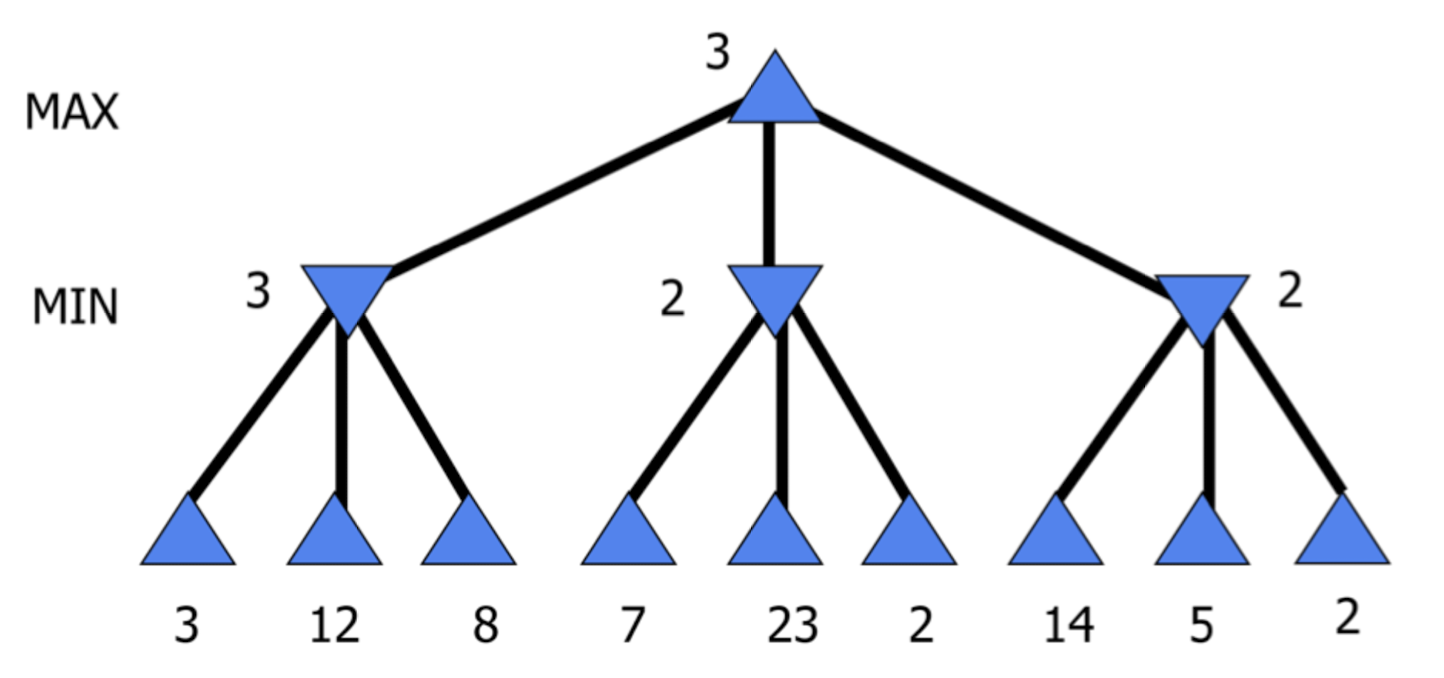
\includegraphics[scale=0.15]{minimax}

\begin{itemize}
    \item Idea: Choose move that yields highest minimax value using DFS
    \item Complete: Yes (if tree is finite)
    \item Time: $O(b^m)$
    \item Space: $O(bm)$
    \item Optimal: Yes (against an optimal opponent)
\end{itemize}

\subsection{Alpha-Beta Pruning}

\begin{itemize}
    \item Motivation: How to save time for Minimax?
    \item Idea: By tracking max. and min. values so far, can prune some paths that we would never choose
    \begin{enumerate}
        \item $\alpha$ contains max. and $\beta$ contains min.
        \item Initially, $\alpha = -\infty$ and $\beta = \infty$
        \item When going down, copy $\alpha$ and $\beta$
        \item Prune if $\alpha \geq \beta$
        \item When going up, depending on MIN/MAX level, update $\alpha$ or $\beta$
    \end{enumerate}
    \item With perfect ordering, time complexity: $O(b^{m/2})$. Doubles search depth.
\end{itemize}

\subsection{Resource Limits}

\begin{itemize}
    \item In reality, search space for games can be very large. $\alpha$-$\beta$ pruning also not fast enough.
    \item Solution: Limit depth (Only see a finite moves ahead) and determine best move using evaluation function to estimate desirability of position (Heuristic)
    \item Other hacks:
    \begin{itemize}
        \item \keyword{Transpoisitions}{Memoize equivalent states}
        \item Pre-computation of opening/closing moves
    \end{itemize}
\end{itemize}

\section{05. Introduction to Machine Learning}

\begin{itemize}
    \item A machine learns if it improves performance P on task T based on experience E. Where T must be fixed, P must be measurable, E must exist
\end{itemize}

\subsubsection{Types of Feedback}

\begin{itemize}
    \item \keyword{Supervised}{Correct answer given for each example}
    \begin{itemize}
        \item \keyword{Regression}{Predict results within continuous output}
        \item \keyword{Classification}{Predict results in discrete output}
    \end{itemize}
    \item \keyword{Unsupervised}{No answers given}
    \item \keyword{Weakly supervised}{Answer given, but not precise}
    \item \keyword{Reinforcement}{Occasional rewards given}
\end{itemize}

\subsection{Decision Trees}

\begin{itemize}
    \item DT can express any function of input attributes, if data is consistent
    \item Goal: Make DT \textbf{compact}. How?
\end{itemize}

\subsubsection{Information Theory}

\begin{itemize}
    \item Idea: Choose attribute that splits examples into subsets that are ideally 'all positive' or 'all negative'
    \item \keyword{Entropy}{Measure of randomness in set of data}
\end{itemize}

\[I(P(v_1), ..., P(v_n)) = - \sum^{n}_{i = 1} P(v_i) \log_{2} P(v_i)\]

\begin{itemize}
    \item For data with $p$ positive examples and $n$ negative examples:
\end{itemize}

\begin{multicols*}{2}
    
    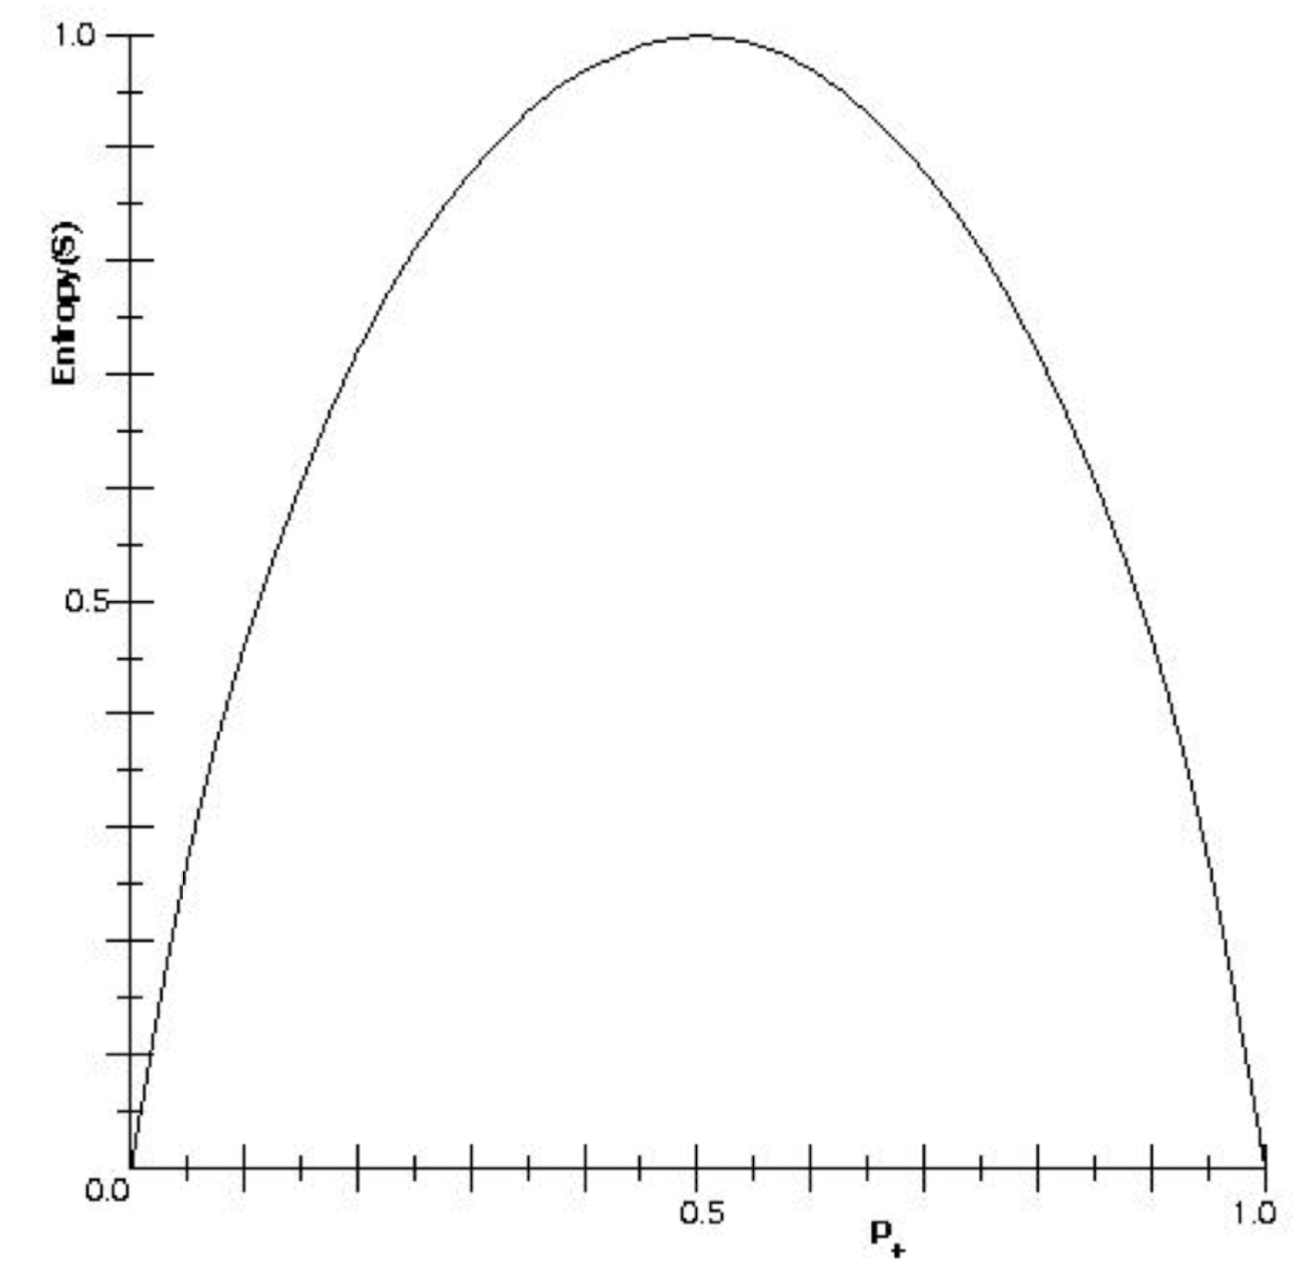
\includegraphics[scale=0.12]{entropy}

    \[I(\frac{p}{p + n}, \frac{n}{p + n}) = \]
    \[- \frac{p}{p + n} \log_{2} \frac{p}{p + n} \]
    \[- \frac{n}{p + n} \log_{2} \frac{n}{p + n}\]

\end{multicols*}

\begin{itemize}
    \item \keyword{Information Gain}{(IG) Reduction in entropy from attribute test} 
    \item Goal: Choose attribute with largest information gain
    \item Intuition: IG = Entropy of this node - Entropy of children nodes
    \item Given chosen attribute $A$ with $v$ distinct values:
\end{itemize}

\[\text{remainder}(A) = \sum_{i = 1}^{v} \frac{p_i + n_i}{p + n} I(\frac{p_i}{p_i + n_i}, \frac{n_i}{p_i + n_i})\]
\[IG(A) = I(\frac{p}{p + n}, \frac{n}{p + n}) - \text{remainder}(A)\]

\begin{itemize}
    \item \keyword{Decision Tree Learning}{Recursively choose attributes with highest IG}
    \item IG is not the only way. Can use whatever objective function that achieves the criteria we want.
\end{itemize}

\subsection{Performance Measurement}

\begin{itemize}
    \item \keyword{Correctness}{Correct if $\hat{y} = y$}
    \item \keyword{Accuracy}{$\frac{1}{m} \sum_{j = 1}^{m} (\hat{y_{j}} = y_{j})$}
\end{itemize}

\begin{multicols*}{2}

    \begin{itemize}
        \item Confusion Matrix:
    \end{itemize}
        
    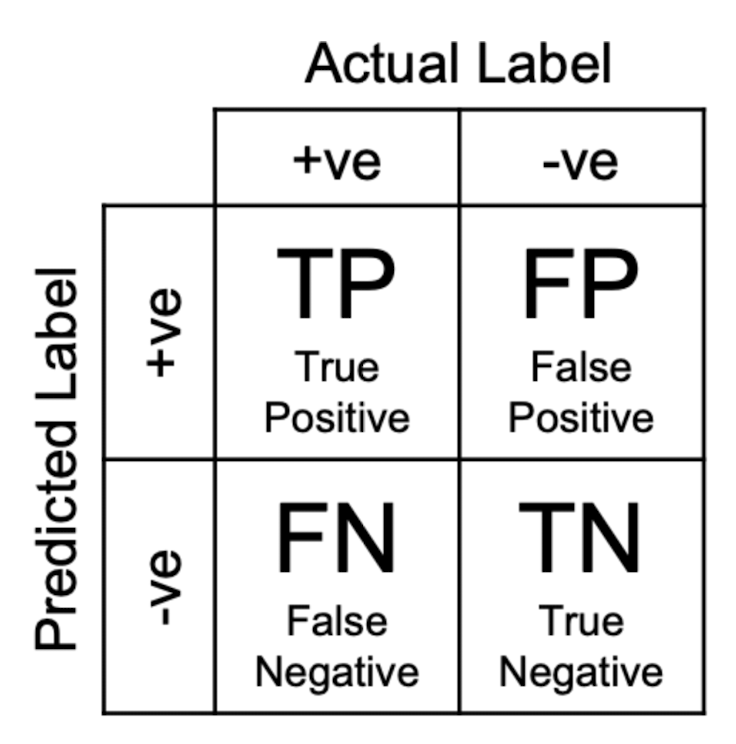
\includegraphics[scale=0.2]{confusion-matrix}

    \begin{itemize}
        \item Accuracy = $\frac{TP + TN}{TP + FN + FP + TN}$
        \item \keyword{Precision}{$\frac{TP}{TP + FP}$} How precise are positive predictions? 
        \item \keyword{Recall}{$\frac{TP}{TP + FN}$} How many actual positives are predicted?
        \item \keyword{F1 Score}{$\frac{2}{1 / P + 1 / R}$} Harmonic mean of precision and recall
    \end{itemize}

\end{multicols*}

\begin{itemize}
    \item Type I Error: FP, Type II Error: FN
    \item FP Rate = $\frac{FP}{FP + TN}$ TP Rate = $\frac{TP}{TP + FN}$
\end{itemize}

\subsection{Pruning}

\begin{itemize}
    \item Motivation: DT overfits to training set, but performs poorly on test set
    \item Occam's Razor: Simple hypothesis preferred
    \item \keyword{Pruning}{Ignores outliers, which reduces overfitting}
    \begin{itemize}
        \item Idea: Go with the majority of T/Fs
        \item E.g. Min-sample, Max-depth
    \end{itemize}
\end{itemize}

\section{06. Linear Regression}

\subsubsection{Notation}

\begin{itemize}
    \item $m$ = Number of training examples
    \item $n$ = Number of features
    \item $x_j ^{(i)}$ = Input feature $j$ of $i$th training example
    \item $y$ = Output variables
\end{itemize}

\subsubsection{Hypothesis}

\[h_w (x): w_0 + w_1 x\]

\subsubsection{Cost Function (Square Error Function)}

\[J(w_0, w_1) = \frac{1}{2m} \sum_{i = 1}^{m} (h_w(x^{(i)}) - y^{(i)})^2\]

\begin{itemize}
    \item Goal: Minimize cost function. Thus, hypothesis is close to training samples
    \item Why squared error? Convenience, since we need to differentiate later
\end{itemize}

\subsection{Gradient Descent}

\begin{enumerate}
    \item Start at some $(w_0, w_1)$. Pick nearby point that reduces $J(w_0, w_1)$.
    \item Repeat until convergence:
\end{enumerate}

\[w_j := w_j - \alpha \frac{dJ(w_0, w_1, ...)}{dw_j}\]

\begin{itemize}
    \item All updates done at end
    \item How to do $\frac{dJ(w_0, w_1)}{dw_j}$? Partial derivative: Hold everything else constant
    \begin{itemize}
        \item $\frac{dJ(w_0, w_1)}{dw_j} = \frac{d}{dw_j} (\frac{1}{2m} \sum_{i = 1}^{m} (w_0 + w_1 x^{(i)} - y^{(i)})^2)$
        \item $\frac{dJ(w_0, w_1)}{dw_0} = \frac{1}{m} \sum_{i = 1}^{m} (w_0 + w_1 x^{(i)} - y^{(i)})$ (Note: Chain rule)
        \item $\frac{dJ(w_0, w_1)}{dw_1} = \frac{1}{m} \sum_{i = 1}^{m} (w_0 + w_1 x^{(i)} - y^{(i)}) x^{(i)}$
    \end{itemize}
    \item Time complexity: $O(kmn)$ where $k$ is number of iterations
\end{itemize}

\subsubsection{Learning Rate}

\begin{itemize}
    \item If $\alpha$ too small, then descent is too slow. If $\alpha$ too big, then might overshoot.
    \item Given constant $\alpha$, descent will grow smaller as we approach minimum
\end{itemize}

\subsubsection{Variants of Gradient Descent}

\begin{itemize}
    \item Batch gradient descent: Consider all training examples when updating
    \item Stochastic gradient descent: Consider 1 random data point at a time (Cheaper and more randomness)
    \item Mini-batch gradient descent
\end{itemize}

\subsubsection{Using Matrices}

\begin{itemize}
    \item Given: $w = 
    \begin{pmatrix}
        w_0\\
        \vdots\\
        w_n
    \end{pmatrix}$ and $x =
    \begin{pmatrix}
        x_0\\
        \vdots\\
        x_n
    \end{pmatrix} = 
    \begin{pmatrix}
        1\\
        \vdots\\
        x_n
    \end{pmatrix}$
    \item $h_w(x): w^T x$
\end{itemize}

\subsubsection{Feature Scaling}

\begin{itemize}
    \item Motivation: Gradient descent does not work well if features have different scales
    \item \keyword{Mean Normalization}{$x_i \leftarrow \frac{x_i - \mu_i}{\sigma_i}$}
\end{itemize}

\subsection{Normal Equation}

\[w = (X^T X)^{-1} X^T Y\]

\begin{itemize}
    \item No need to choose $\alpha$ and feature scaling
    \item $X^T X$ needs to be invertible
    \item Time complexity: $O(n^3)$. Slow if $n$ is big
\end{itemize}

\section{07. Logistic Regression}

\begin{itemize}
    \item Motivation: Classification with continuous input values. 
    \item Idea: Come up with a decision boundary to separate data points. $h_w (x_1, x_2) = 1$, if $w_0 + w_1 x_1 + w_2 x_2 > 0$, or $0$, otherwise
\end{itemize}

\subsection{Sigmoid Function}

\begin{itemize}
    \item Motivation: Step function is discontinuous and not differentiable
\end{itemize}

\begin{multicols*}{2}
    
    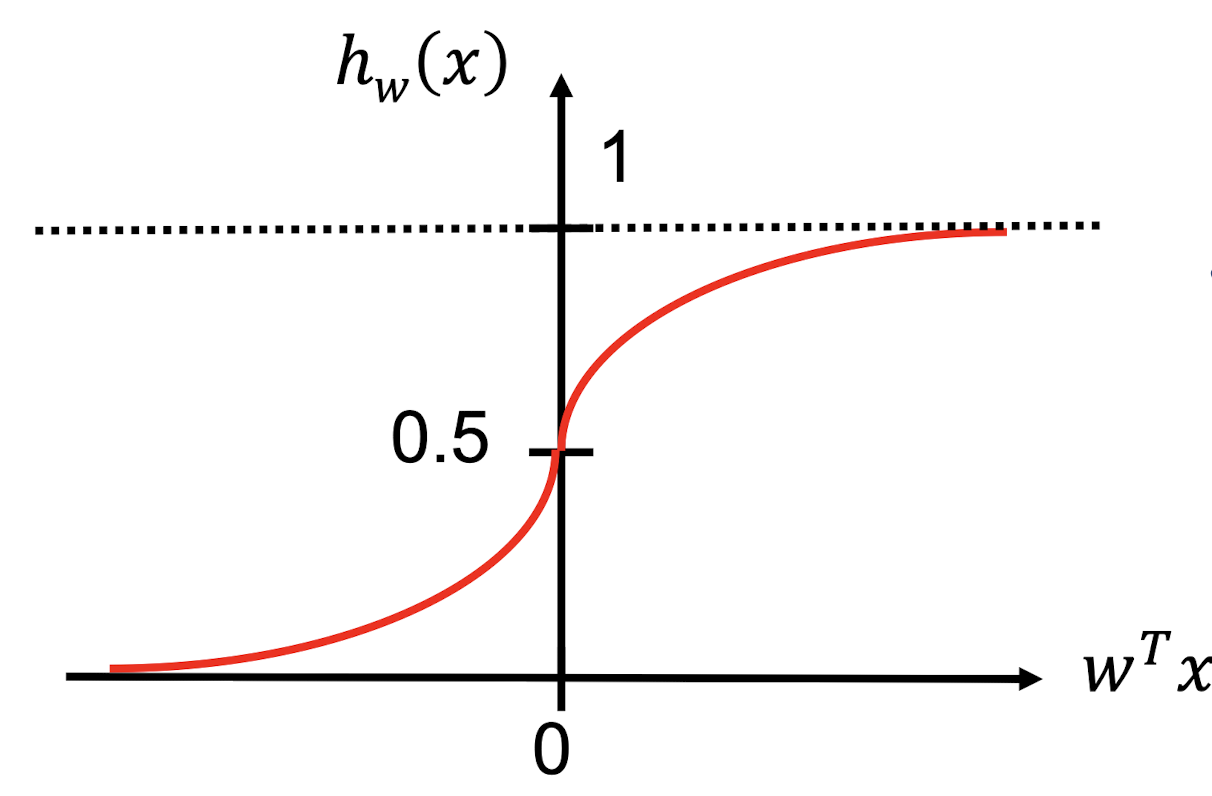
\includegraphics[scale=0.16]{sigmoid-function}

    \[h_w (x) = g(w^T x)\]

    \[g(z) = \frac{1}{1 + e^{-z}}\]

\end{multicols*}

\subsubsection{Hypothesis}

\[h_w (x): \frac{1}{1 + e^{-w^T x}}\]

\begin{itemize}
    \item Interpretation: Estimated probability that $y = 1$ given input $x$
\end{itemize}

\subsubsection{Cost Function}

\begin{itemize}
    \item Problem: Least square error gives non-convex cost function, which is bad for G.D.
    \item Solution: Use $log$
\end{itemize}

\begin{multicols*}{2}

    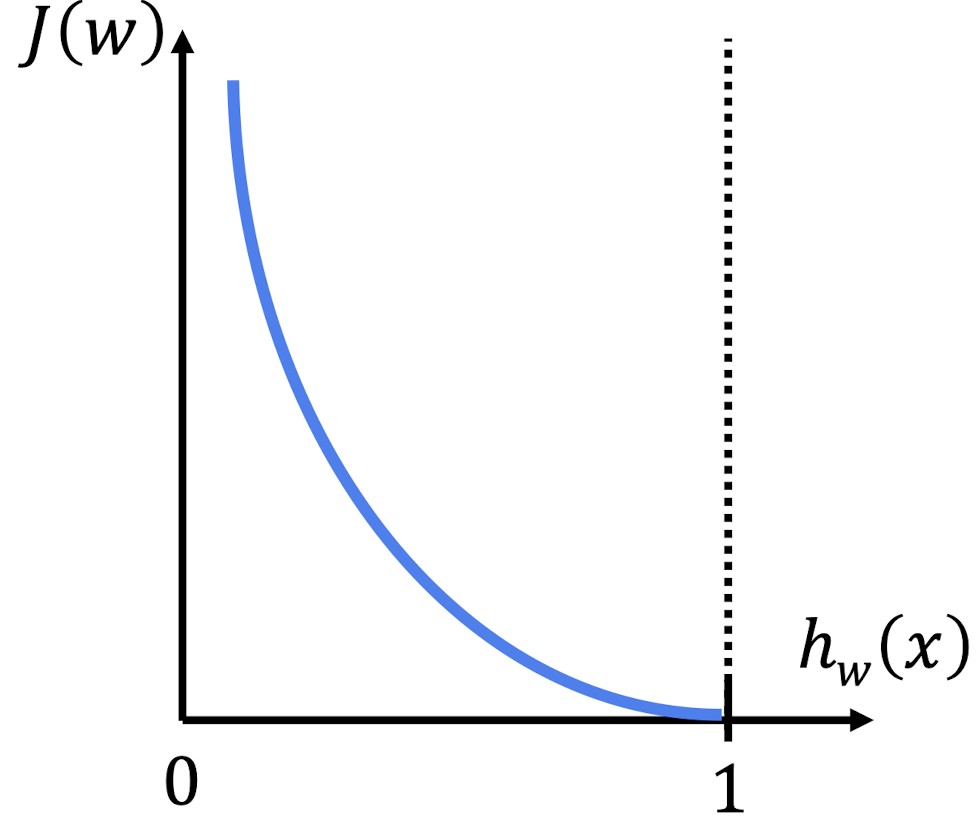
\includegraphics[scale=0.13]{logistic-regression-cost-1}

    \begin{itemize}
        \item If $y = 1$, let cost be $-log(h_w (x))$
        \begin{itemize}
            \item $h_w (x) \rightarrow 0, J(w) \rightarrow \infty$
            \item $h_w (x) \rightarrow 1, J(w) \rightarrow 0$
        \end{itemize}
    \end{itemize}

\end{multicols*}

\begin{multicols*}{2}

    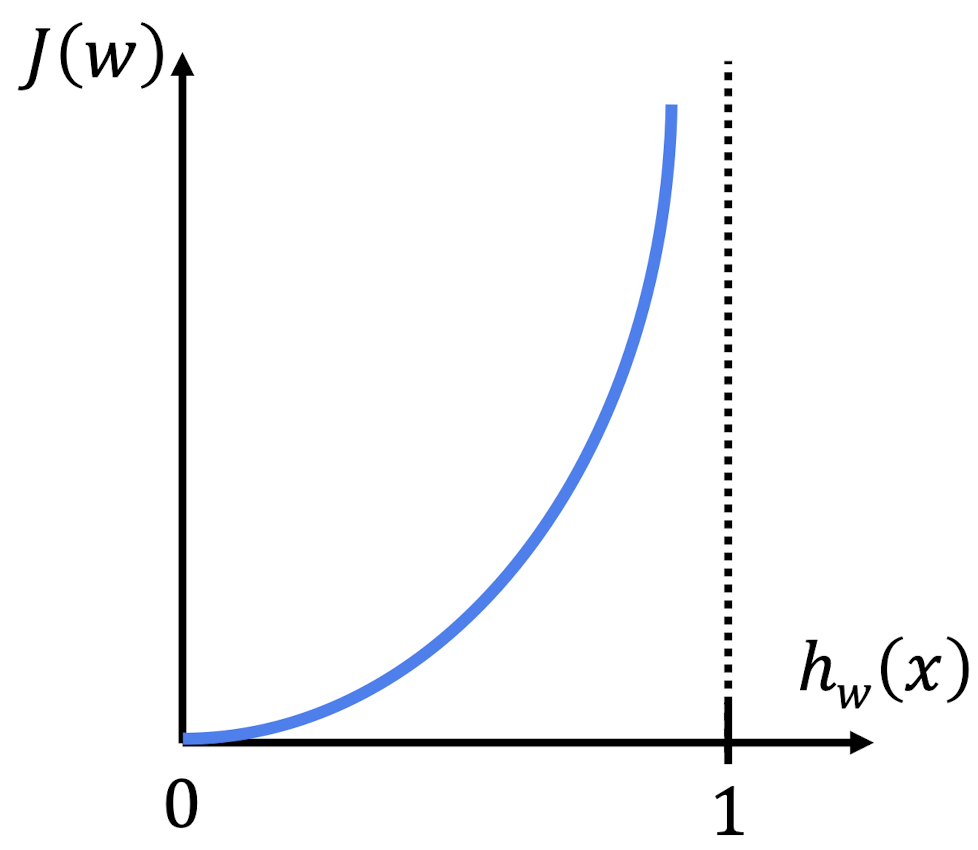
\includegraphics[scale=0.13]{logistic-regression-cost-2}

    \begin{itemize}
        \item If $y = 0$, let cost be $-log(1 - h_w (x))$
        \begin{itemize}
            \item $h_w (x) \rightarrow 0, J(w) \rightarrow 0$
            \item $h_w (x) \rightarrow 1, J(w) \rightarrow \infty$
        \end{itemize}
    \end{itemize}

\end{multicols*}

\[J(w) = - \frac{1}{m} \sum_{i=1}^{m} y^{(i)} log h_w (x^{(i)}) + (1 - y^{(i)}) log (1 - h_w (x^{(i)}))\]

\subsubsection{Gradient Descent}

\begin{itemize}
    \item Same algorithm as linear regression
    \item $\frac{d J(w)}{d w_j} = \frac{1}{m} \sum_{i=1}^{m} (h_w (x^{(i)}) - y^{(i)}) x_{n}^{(i)}$ (Same as linear regression)
\end{itemize}

\subsection{Multi-class Classification}

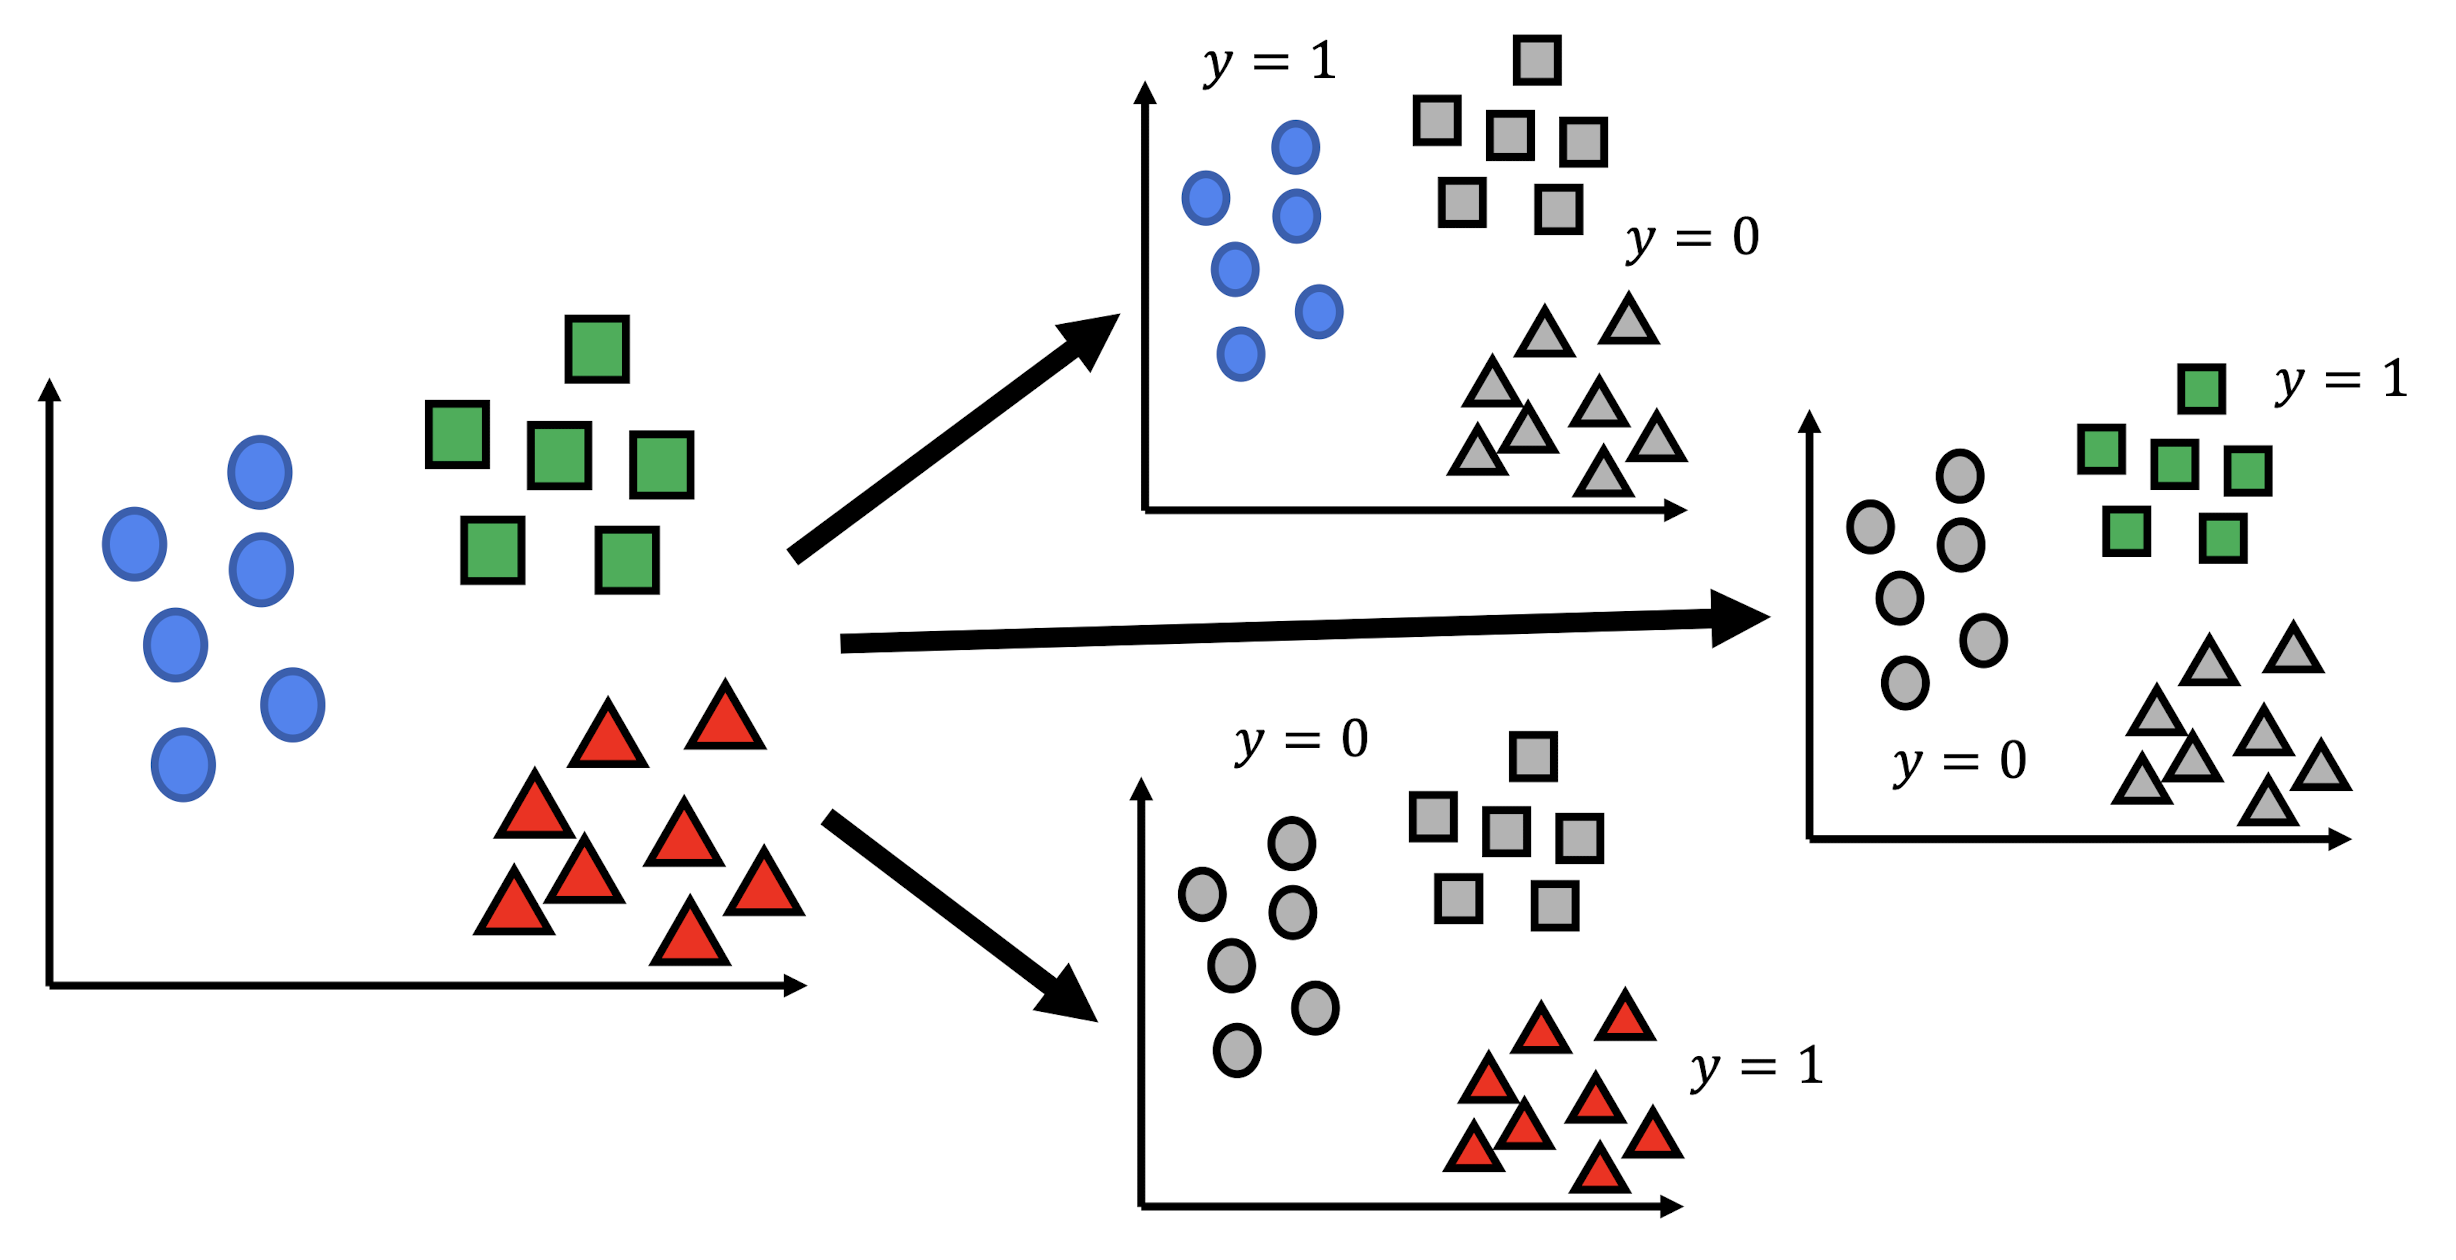
\includegraphics[scale=0.15]{multi-class-classification}

\begin{enumerate}
    \item Train binary classifier $h_{w}^{(i)}(x)$ for each class $i$ to predict $y = i$
    \item For each input $x$, pick class $i$ is greatest (i.e. $\max_i h_{w}^{(i)} (x)$)
\end{enumerate}

\section{08. Model Evaluation and Selection}

\subsubsection{Linear Regression}

\[J_{\text{test}}(w) = \frac{1}{2m_{\text{test}}} \sum_{i=1}^{m_{\text{test}}} (h_w (x_{\text{test}}^{(i)}) - y_{\text{test}}^{(i)})^2\]

\subsubsection{Logistic Regression}

\[
    \text{error} (h_w(x), y) = 
    \begin{cases}
        1 & \text{if misclassification} \\
        0 & \text{otherwise}
    \end{cases}
\]

\[\text{Test Error} = \frac{1}{m_{\text{test}}} \sum_{i=1}^{m_{\text{test}}} \text{error}(h_w (x_{\text{test}}^{(i)}), y_{\text{test}}^{(i)})\]

\subsubsection{Model Selection}

\begin{itemize}
    \item How to choose model? (i.e. $x^2$, $x^3$, etc. for hypothesis)
    \begin{enumerate}
        \item Split data into 3 sets: Training set, validation set, and test set
        \item Train each model using training set
        \item Compute $J_{cv}(w)$ for each model and pick model with lowest $J_{cv}(w)$
        \item Use $J_{\text{test}}(w)$ to estimate performance on unseen samples
    \end{enumerate}
\end{itemize}

\subsubsection{Bias and Variance}

\begin{itemize}
    \item \keyword{High bias}{Underfit}, \keyword{High variance}{Overfit}
    \item As degree of polynomial increases:
\end{itemize}

\begin{multicols*}{2}
    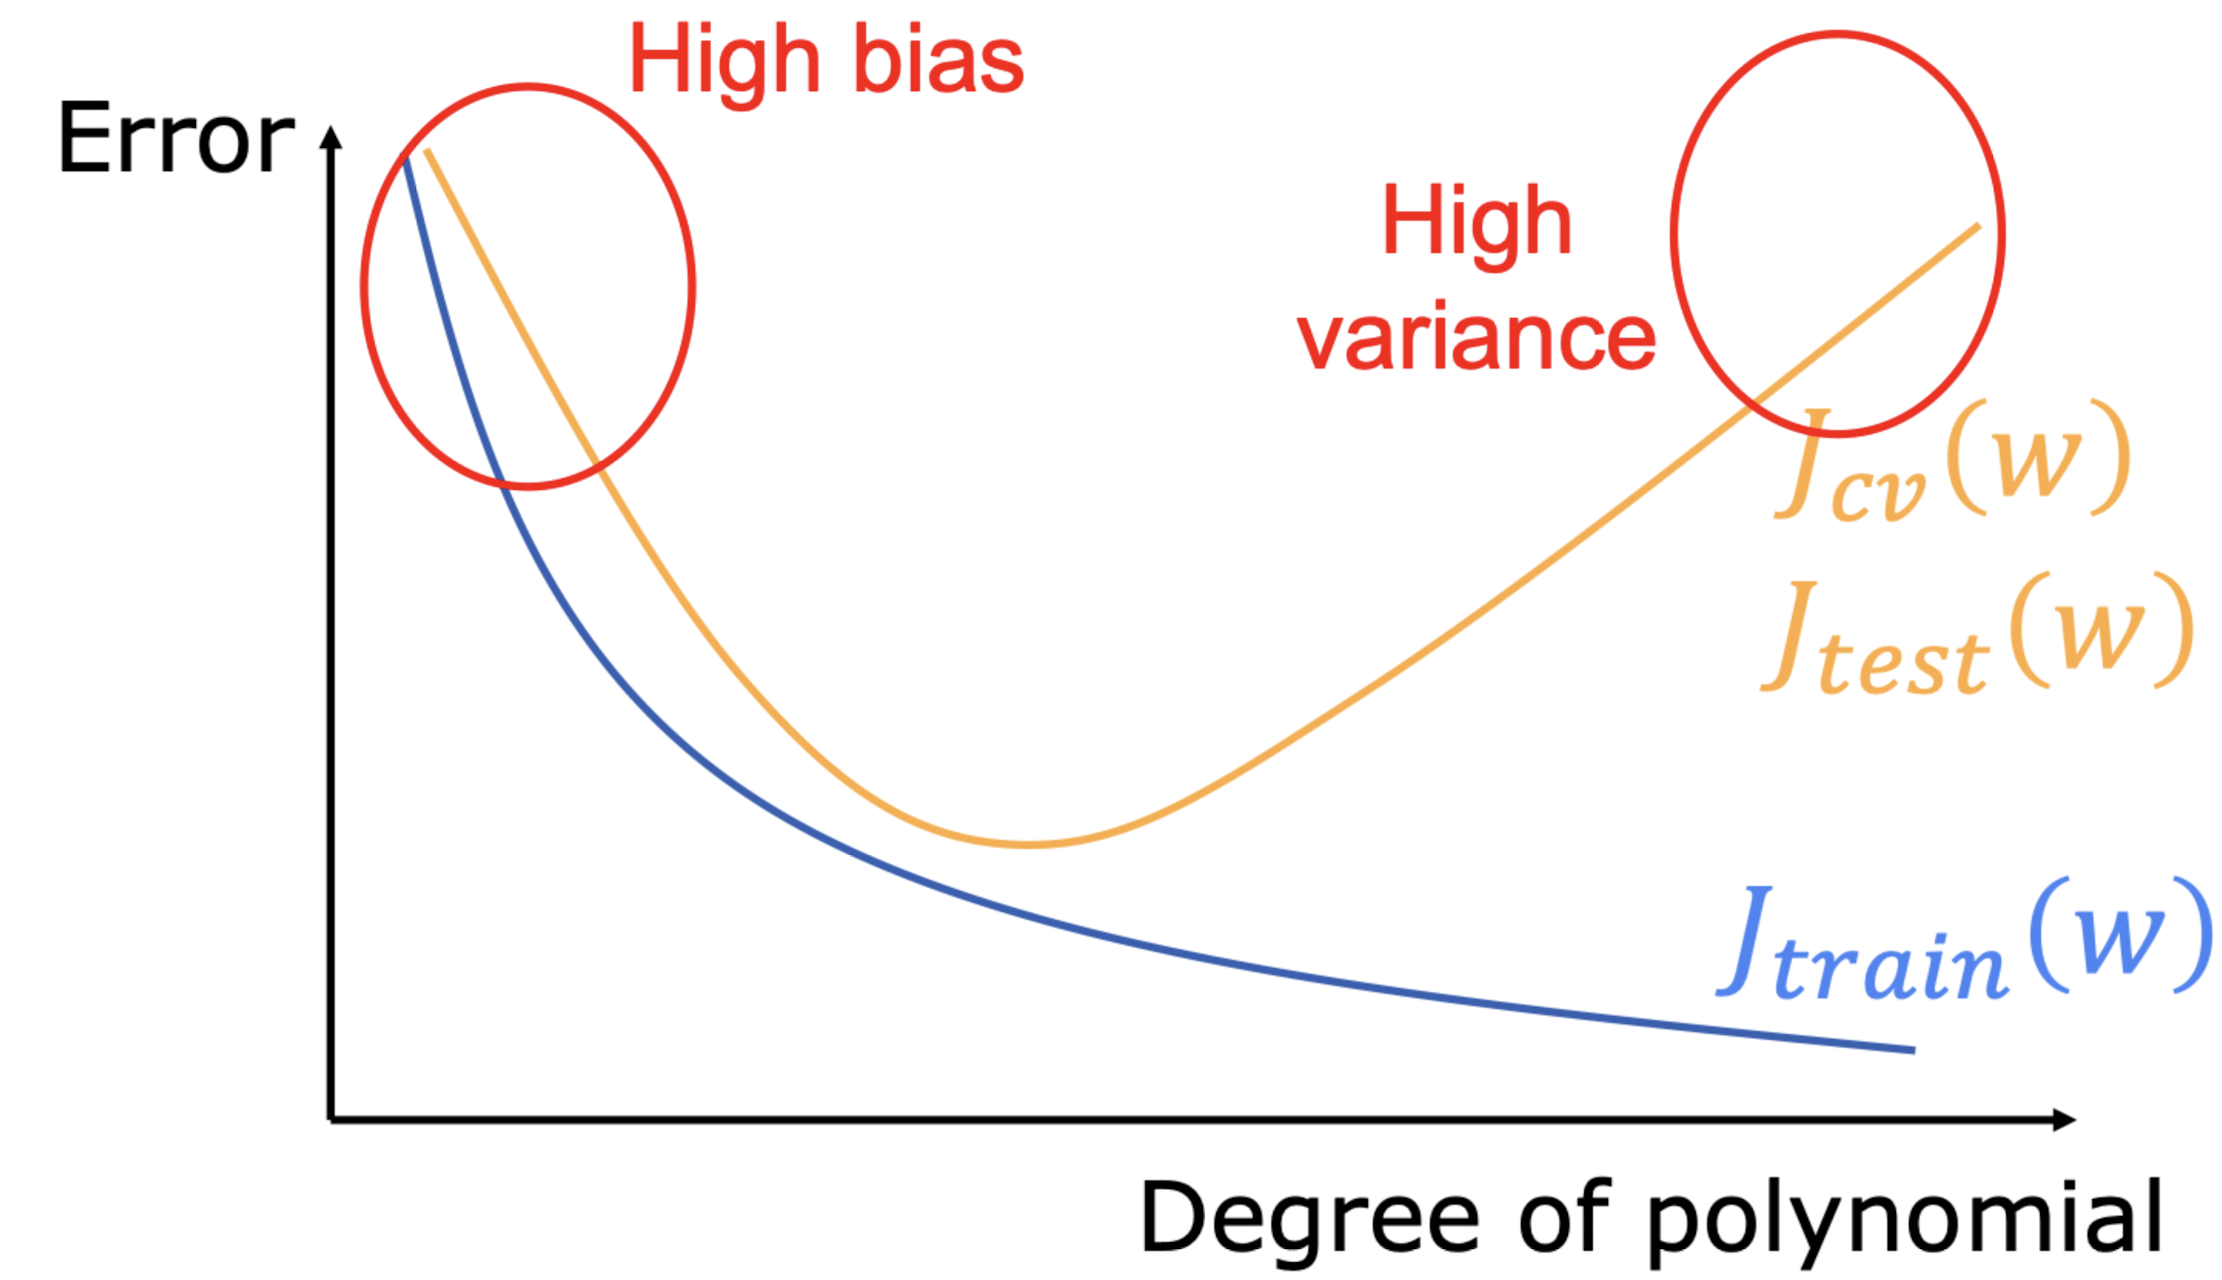
\includegraphics[scale=0.1]{bias-and-variance}

    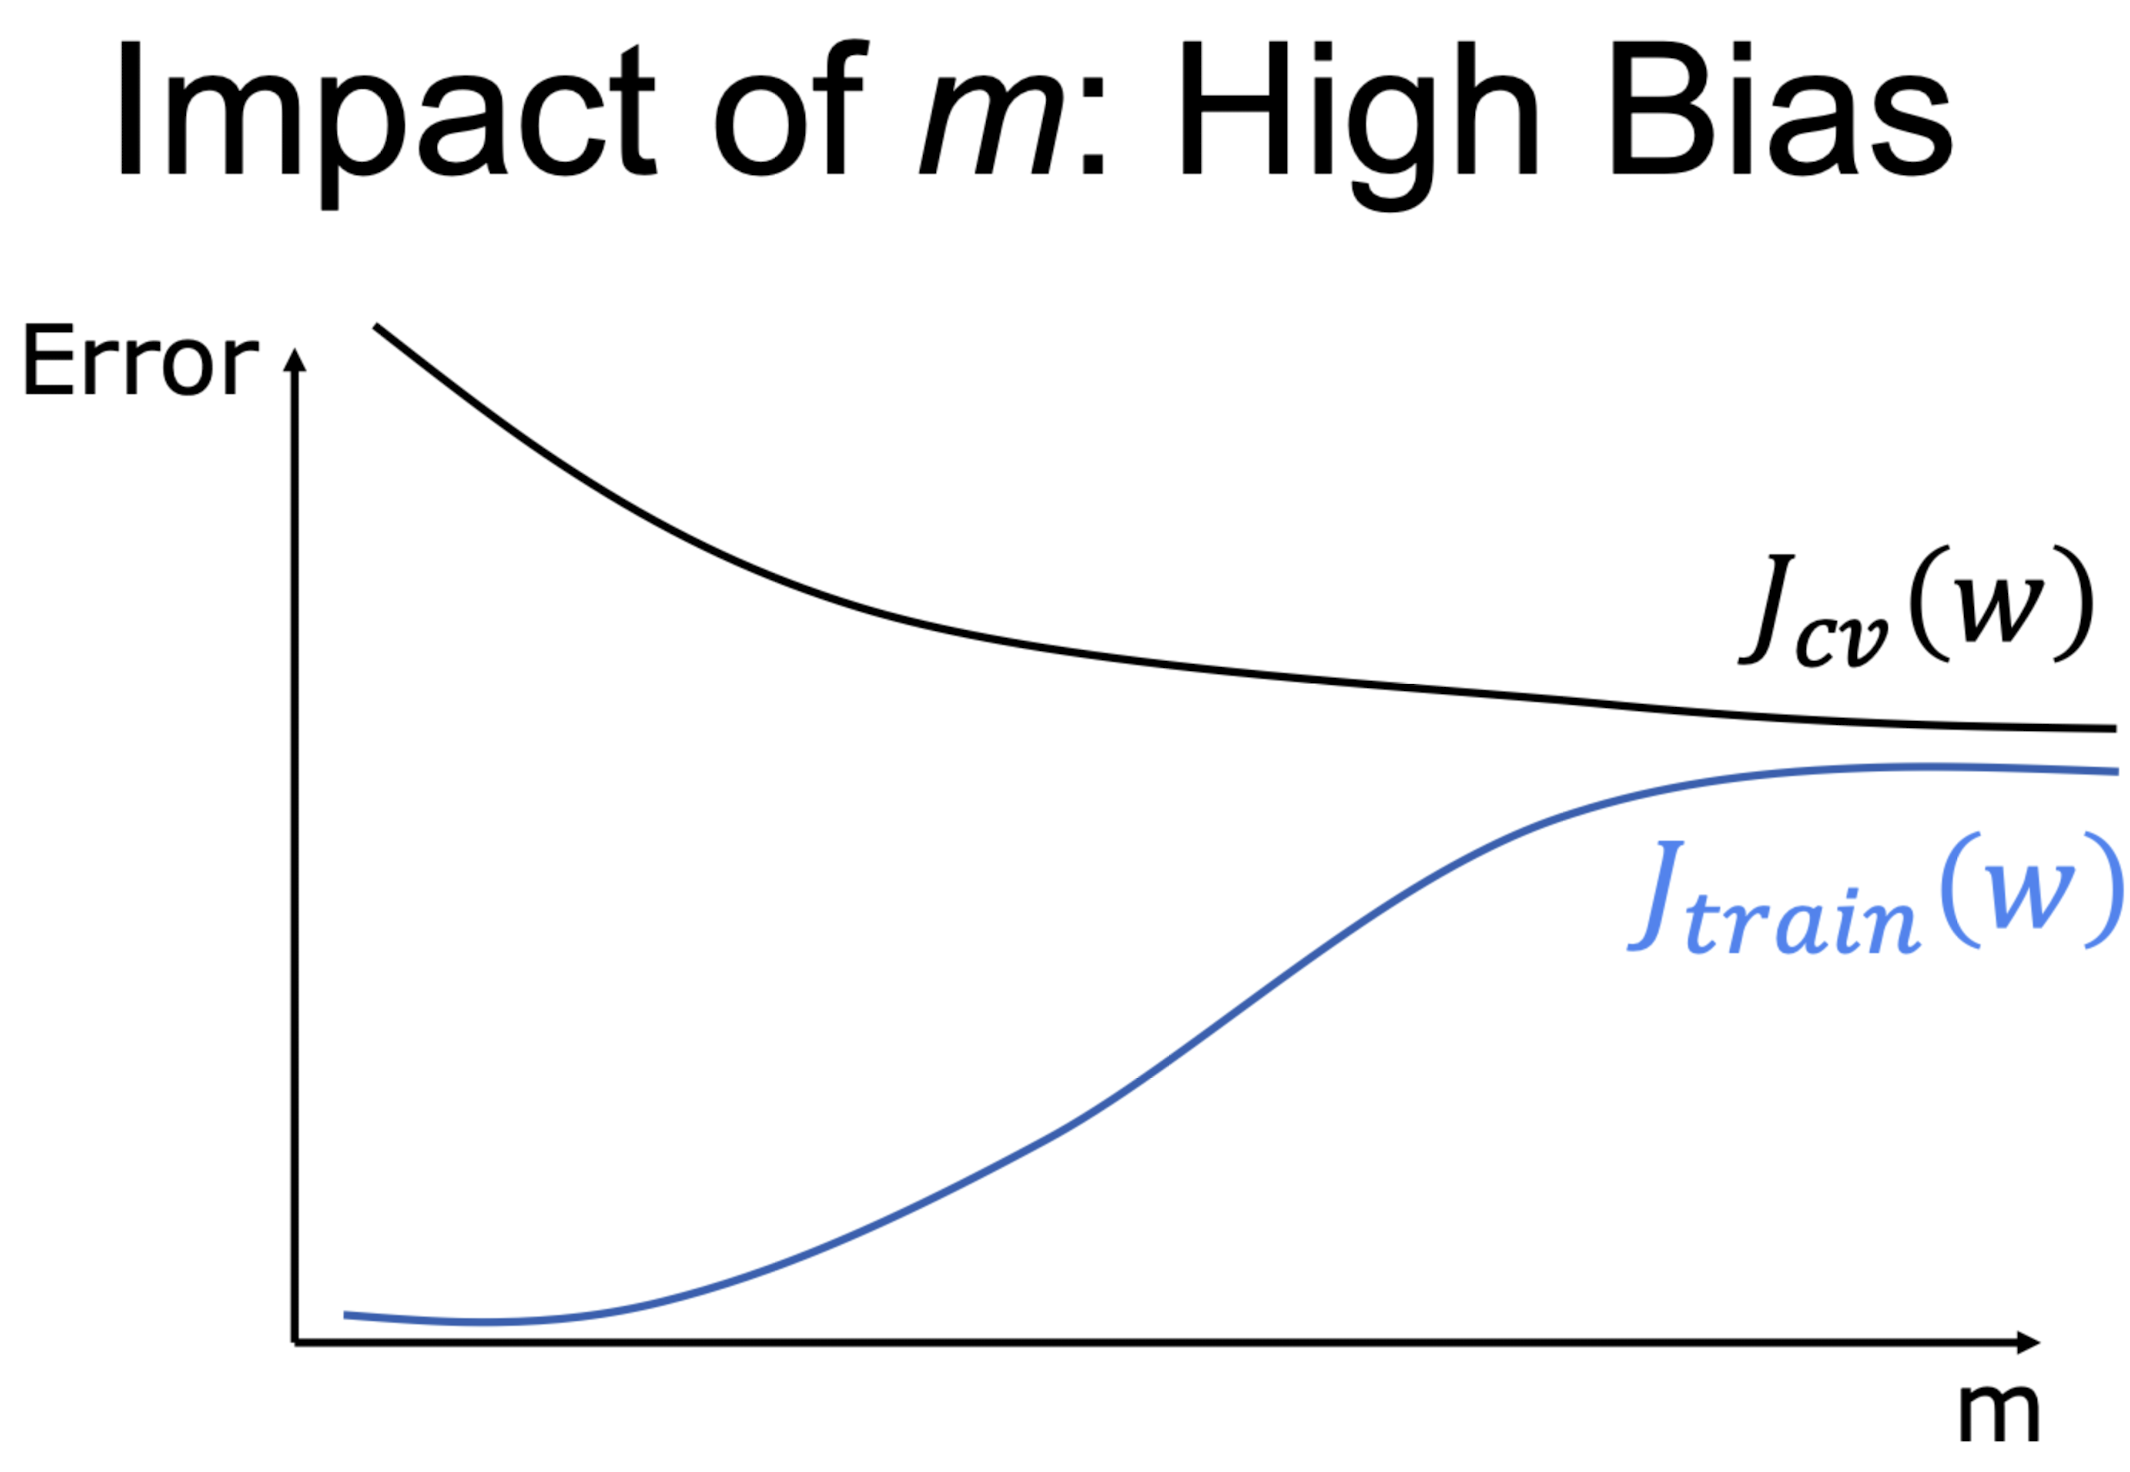
\includegraphics[scale=0.1]{high-bias} 

    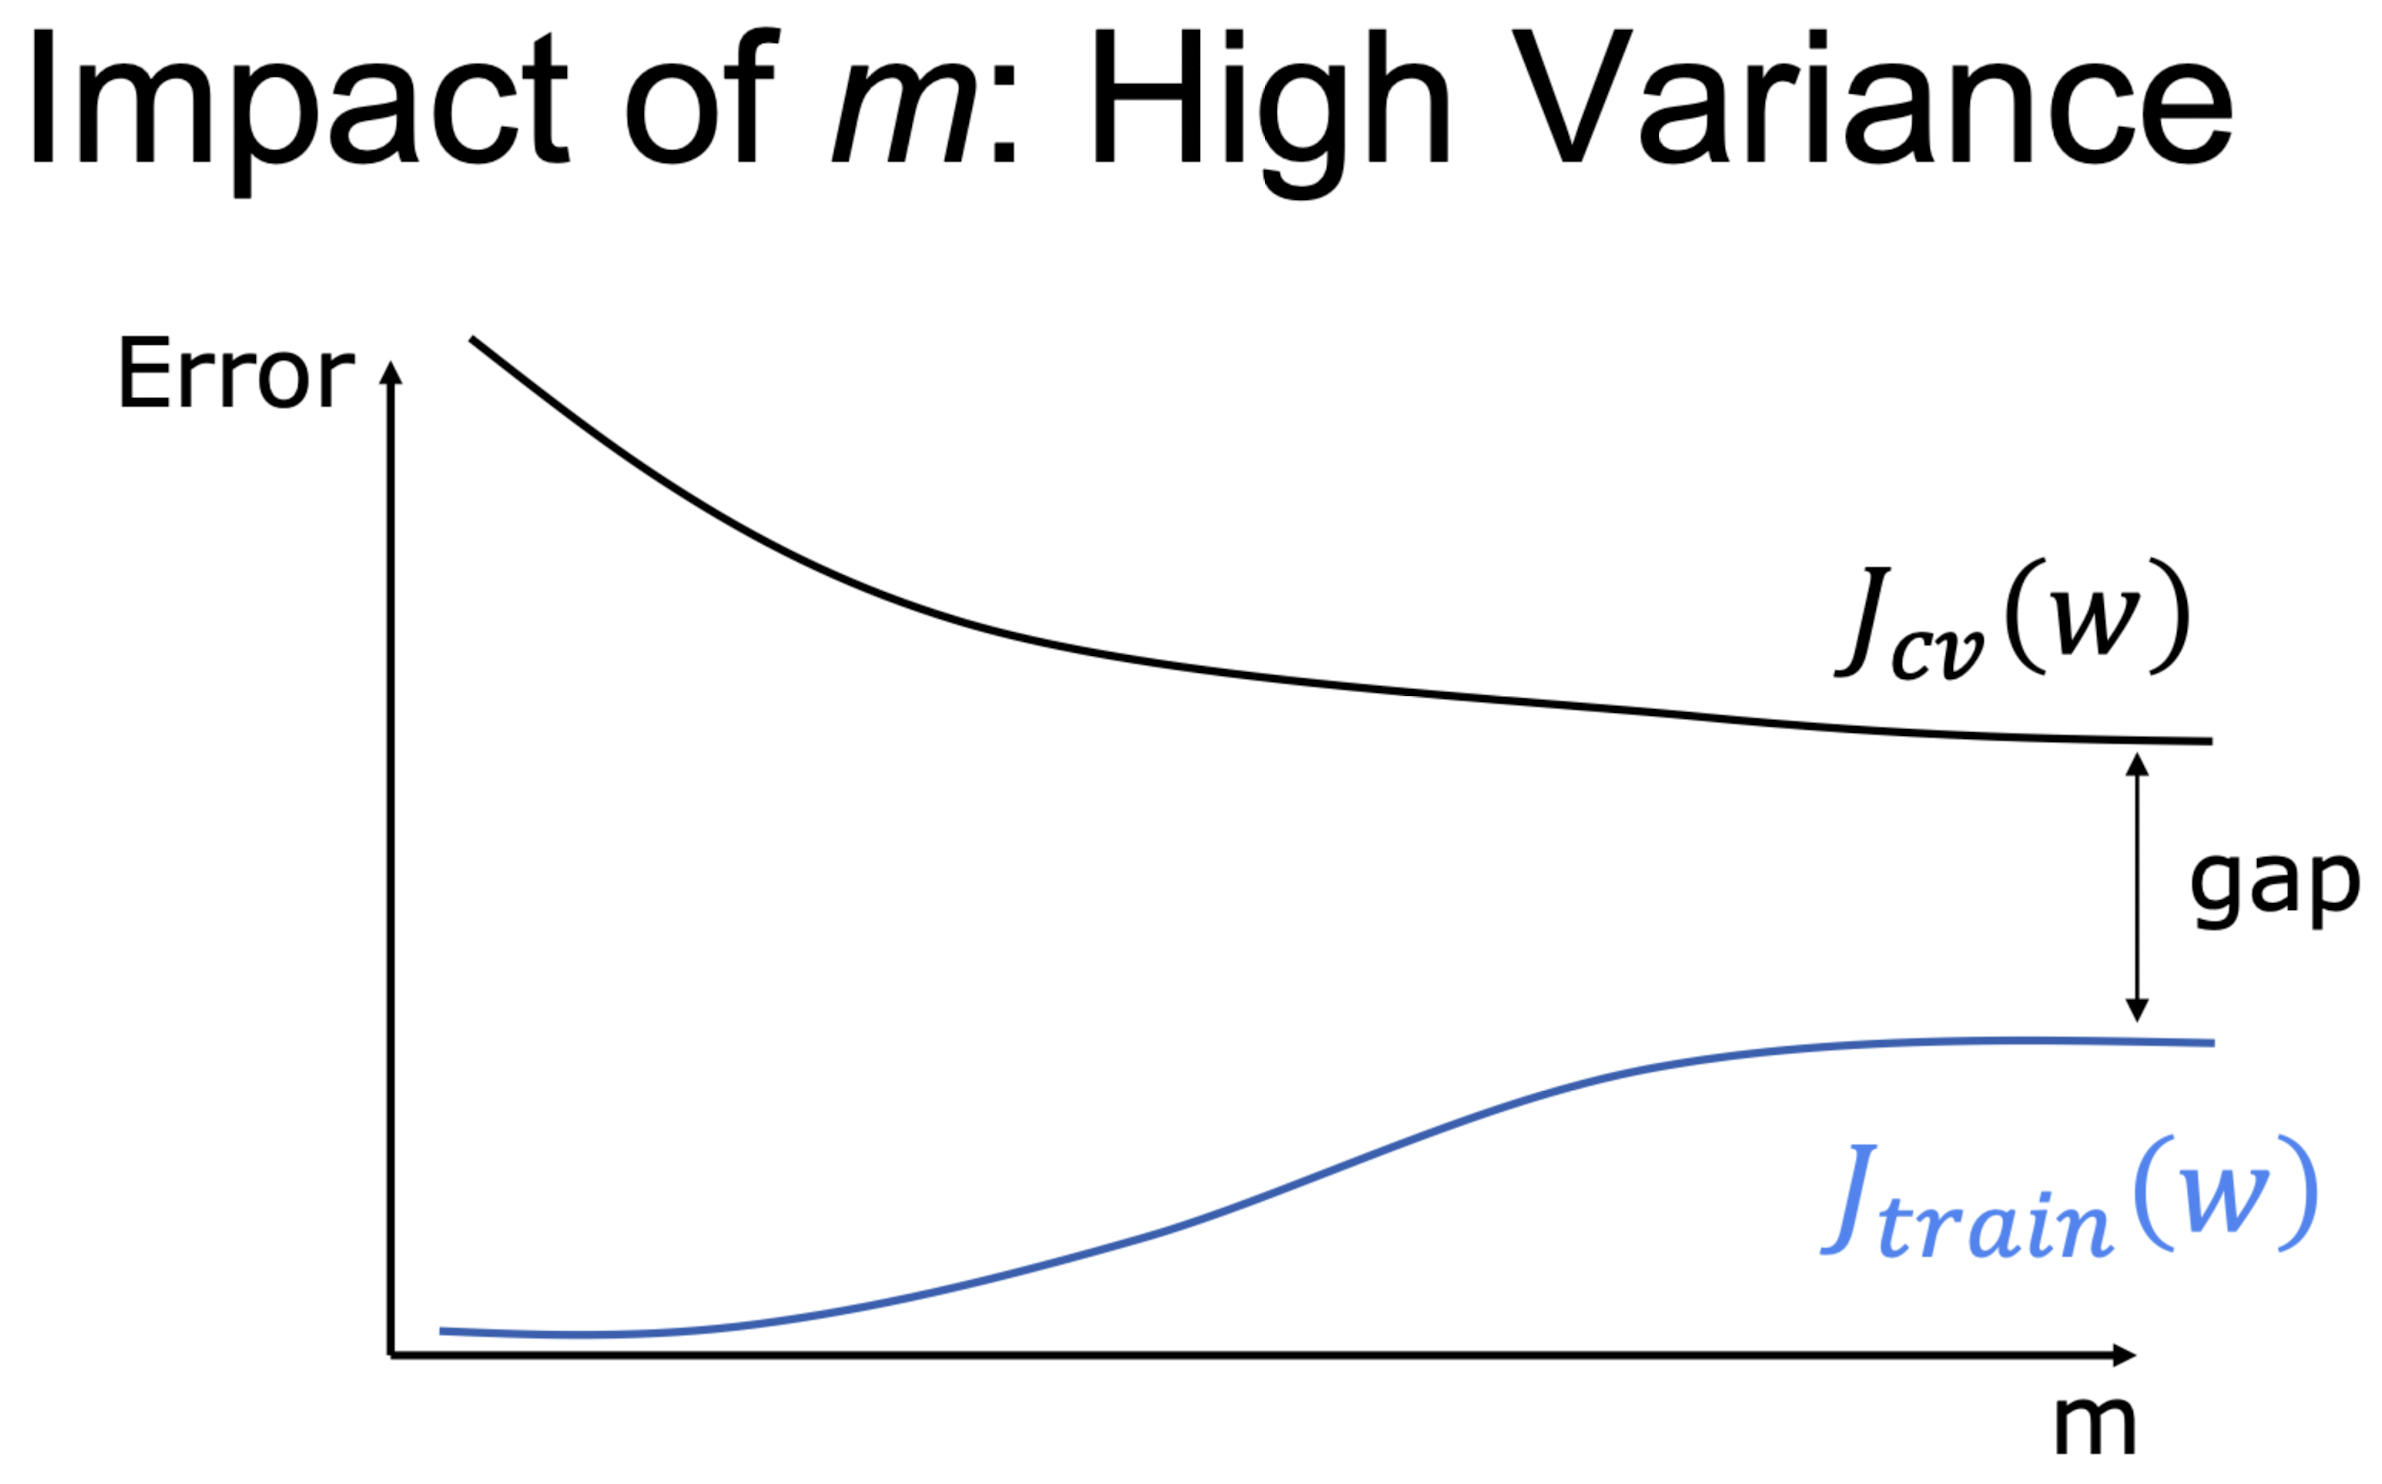
\includegraphics[scale=0.09]{high-variance} 

    \begin{itemize}
        \item Observation: If high bias, $J_{cv}$ and $J_{train}$ are equally bad (Small gap). If high variance, more samples does not help close the gap.
        \item How do we address overfitting?
        \begin{itemize}
            \item Reduce number of features
            \item \keyword{Regularization}{Keep features, but reduce respective weights}
        \end{itemize}
    \end{itemize}
\end{multicols*}

\section{09. Regularization}

\begin{itemize}
    \item Idea: Include $w$ inside $J(w)$ to minimize weights and get simpler hypothesis
    \item What if $\lambda$ is too large? Weights tend to 0, resulting in straight line
    \item How to choose $\lambda$? Use validation set
    \begin{itemize}
        \item Small $\lambda$: $J_{\text{train}}(w)$ low and $J_{cv}(w)$ high (Overfit)
        \item Large $\lambda$: $J_{\text{train}}(w)$ high and $J_{cv}(w)$ high (Underfit)
    \end{itemize}
\end{itemize}

\subsubsection{Linear Regression with Regularization}

\[J(w) = \frac{1}{2m} (\sum_{i = 1}^{m} (h_w(x^{(i)}) - y^{(i)})^2 + \lambda \sum_{i=1}^{n} w_i^2)\]

\[w_n := w_n - \frac{\alpha}{m} \sum_{i=1}^{m} ((h_w(x^{(i)}) - y^{(i)})x_n^{(i)}) - \frac{\alpha \lambda}{m} w_n\]

\subsubsection{Logistic Regression with Regularization}

\[J(w) = - \frac{1}{m} \sum_{i = 1}^{m} y^{(i)} log(h_w(x^{(i)})) + (1 - y^{(i)})log(1 - h_w(x^{(i)})) + \frac{\lambda}{2m} \sum_{i=1}^{n} w_i^2\]

\[w_n := w_n - \frac{\alpha}{m} \sum_{i=1}^{m} ((h_w(x^{(i)}) - y^{(i)})x_n^{(i)}) - \frac{\alpha \lambda}{m} w_n\]

\[w = (X^T X + \lambda I)^{-1} X^T Y \text{ where $I$'s first column is 0}\]

\begin{itemize}
    \item $X^T X$ can be non-invertible
\end{itemize}

\section{10. Support Vector Machine}

\begin{itemize}
    \item Idea: Maximize margin between positive and negative samples
\end{itemize}

\subsubsection{Decision Rule}

\[w \cdot x \geq c \rightarrow \text{Positive}; w \cdot x < c \rightarrow \text{Negative}\]

\begin{itemize}
    \item Dot product: $u \cdot v = u^T v = p ||v||$ (By law of cosine)
    \item Intuition: Decision boundary $\perp$ Weight vector. $w \cdot x = p ||w||$. Sample $a$ is on decision boundary if $w \cdot a = c$
    \item Constraints: $\text{Let } b = -c$
    \begin{itemize}
        \item $w \cdot x + b \geq 1 \text{ if } y = 1$
        \item $w \cdot x + b < -1 \text{ if } y = 0$
        \item Combined: Let $\hat{y}^{(i)} = 1 \text{ or } -1$ for pos. and neg. samples respectively. $\hat{y}^{(i)} (w \cdot x^{(i)} + b) \geq 1$
        \item If $x$ is inside margin, then $w \cdot x + b = 1 \text{ or } -1$ respectively
        \item Why add these constraints? Mathematical convenience for hinge loss
    \end{itemize}
\end{itemize}

\subsubsection{Margin}

\[\text{Margin width} = \frac{2}{||w||}\]

\begin{itemize}
    \item Let $x^+$ and $x^-$ be closest positive and negative samples
    \item Margin width = $(x^+ - x^-) \cdot \frac{w}{||w||}$ (i.e. Length of projection of $x^+ - x^-$ on weight vector) $= \frac{1 - b + 1 + b}{||w||}$ (since $x^+$ and $x^-$ are inside margin) $= \frac{2}{||w||}$ 
\end{itemize}

\subsubsection{Objective Function for Hard-Margin}

\[\min \frac{1}{2} ||w||^2 \text{ s.t. } \hat{y}^{(i)} (w \cdot x + b \geq 1)\]

\begin{enumerate}
    \item Maximize margin: $\max \frac{2}{||w||} = \min ||w|| = \min \frac{1}{2} ||w||^2$
    \item Classify correctly
\end{enumerate}

\begin{itemize}
    \item \keyword{Hard-Margin}{No samples inside margin}
    \item Before, we assume hard margin. What if there exists outliers that causes SVM to overfit?
\end{itemize}

\subsubsection{Objective Function for Soft-Margin}

\[
    h_w (x) = 
    \begin{cases}
        1 & \text{if } w^T x \geq 0 \\
        0 & \text{otherwise} 
    \end{cases}
\]

\begin{itemize}
    \item \keyword{Slack Variable}{($\xi$) Loss of misclassified point}
    \item Goal: Maximize margin and allow misclassification by tweaking $C$
    \begin{itemize}
        \item Large $C$ overfits (Basically hard-margin). Small $C$ underfits.
        \item i.e. $\min (\frac{1}{2} ||w||^2 + C \sum_i \xi^{(i)}) \text{ s.t. } \forall i, \xi^{(i)} \geq 0 \text{ and } \hat{y}^{(i)}(w \cdot x^+ b) \geq 1 - \xi^{(i)} \rightarrow J(w) = C \sum_i \max(0, 1 - \hat{y}^{(i)} (w^T x^{(i)})) + \frac{1}{2} \sum_{i=1}^{n} w_{i}^{2}$
        \item Hard-margin: Must follow constraint. Soft-margin: Constraint is flexible with slack variable, so can define cost function to minimize.
    \end{itemize}
\end{itemize}

\[J(w) = C \sum_{i}^{m} y^{(i)} \text{cost}_1 (w^T x^{(i)}) + (1 - y^{(i)}) \text{cost}_0 (w^T x^{(i)}) + \frac{1}{2} \sum_{i=1}^{n} w_{i}^{2}\]

\begin{multicols*}{2}

    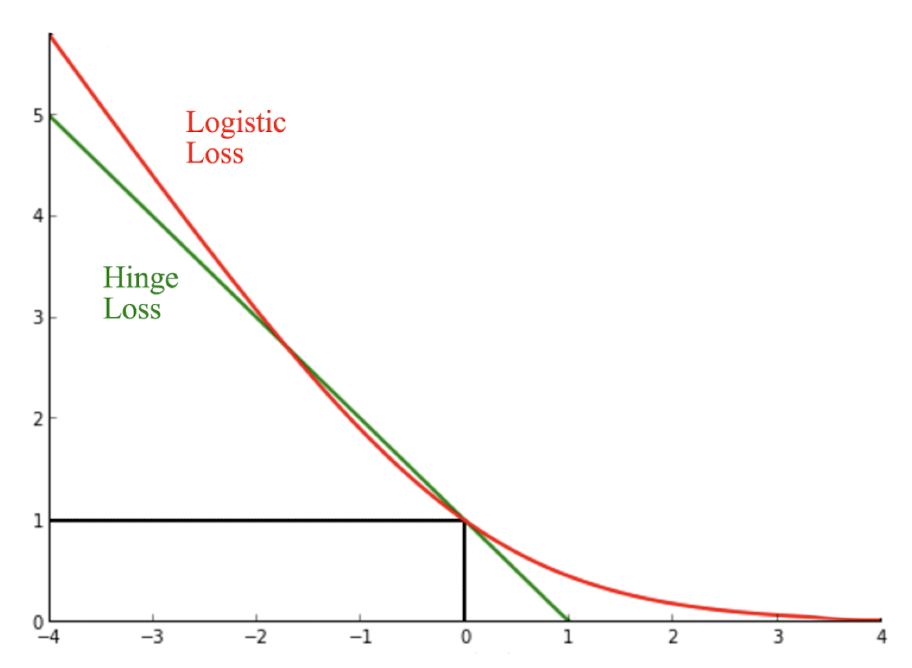
\includegraphics[scale=0.15]{hinge-loss}
    
    \begin{itemize}
        \item \ilkeyword{Hinge Loss}
        \begin{itemize}
            \item $\text{cost}_1 (z) = \max(0, 1 - z)$
            \item $\text{cost}_0 (z) = \max(0, 1 + z)$
        \end{itemize}
    \end{itemize}

\end{multicols*}

\subsection{Kernel}

\begin{itemize}
    \item Motivation: What if data is not linearly separable?
    \item Idea: Map features to higher dimensions (i.e. $\phi (x)$). High dim. is slow.
    \item \keyword{Kernel Function}{Dot product between two points in transformed dim.}
\end{itemize}

\[K(u, v) = \phi(u) \cdot \phi(v)\]

\begin{itemize}
    \item Property: Getting $K(u, v)$ does not need $\phi(u)$ and $\phi(v)$
    \item \keyword{Linear Kernel}{$K(u, v) = u \cdot v$}
    \item \keyword{Polynomial Kernel}{$K(u, v) = (u \cdot v)^d$}
    \item \keyword{Gaussian Kernel}{$K(u, v) = e^{- ||u - v||^2 / 2 \sigma ^2}$} (Note: $\phi(u)$ can map to infinite dimensions)
\end{itemize}

\subsubsection{Kernel Trick}

\begin{itemize}
    \item By manipulating SVM objective func. and decision rule, $x^{(i)} \cdot x^{(j)}$ emerges
    \item If we map features (i.e. $\phi(x)$), can replace above term with kernel ($K(u, v)$)
    \item Trick: No need to compute transformed features explicitly
\end{itemize}

\subsubsection{Similarity Features}

\begin{itemize}
    \item Idea: Compute new features based on proximity to landmarks
    \item Given example $x$. $f_i = sim (x, l^{(i)}) = K(x, l^{(i)})$ where $K$ is gaussian kernel
    \item Transformed x: $f = [f_0, f_1, \dots, f_m]^T$. Plug into obj. function.
    \item Do feature scaling, else similarity value may be dominated by some features
    \item Large $\sigma$ underfits (Smoother features). Small $\sigma$ overfits.
    \item Not all similarity functions get valid kernels. Need to satisfy Mercer's Thm.
\end{itemize}

\section{11. Neural Networks}

\begin{itemize}
    \item Idea: Models after human brain (Perceptron)
\end{itemize}

\begin{multicols*}{2}
    
    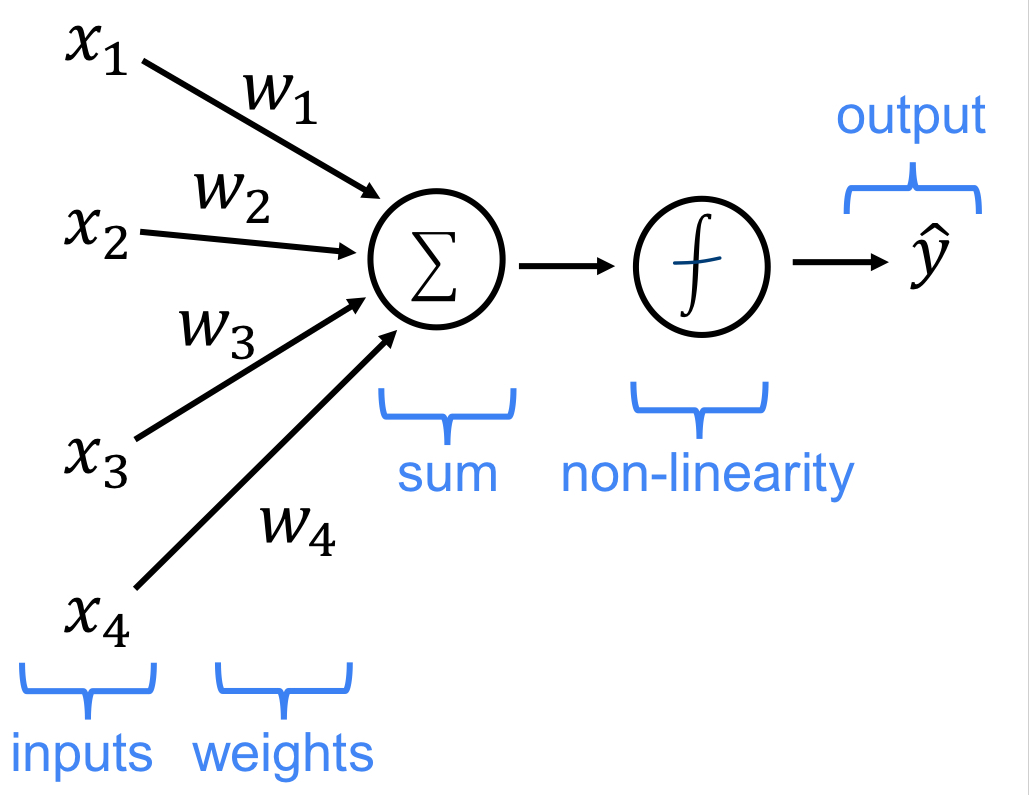
\includegraphics[scale=0.1]{perceptron}

    \[\hat{y} = g(\sum_{i = 0}^{n} w_i x_i) \text{ where } x_0 = 1\]

    \begin{itemize}
        \item \keyword{Activation Function}{($g$) Non-linear function (e.g. Step func. $sgn(x)$, $\sigma(x)$, $tanh(x)$, $max(0, x)$)}
    \end{itemize}

\end{multicols*}

\begin{itemize}
    \item Supports both classification and regression. Depends on activation func.
    \begin{itemize}
        \item If activation function is linear, then regression
    \end{itemize}
\end{itemize}

\subsection{Perceptron Learning Algorithm (PLA)}

\begin{enumerate}
    \item Initialize weights $w$
    \item Select misclassified sample and update $w$. Repeat until convergence.
\end{enumerate}

\[w \leftarrow w + \eta (y - \hat{y})x\]

\begin{itemize}
    \item Why this works? Each update gets closer to correct classification
    \item Different from GD!
    \item Ends when no more misclassification. Thus, can select any linear model
    \item Cannot converge on non-linear data
\end{itemize}

\subsection{Single-Layer Neural Network}

\begin{itemize}
    \item Basically logistic regression, if activation function is $\sigma(x)$
    \item How to determine weights? Gradient descent
    \begin{itemize}
        \item Many ways to calculate error. e.g. MSE ($J(w) = \frac{1}{2} (\hat{y} - y)^2$).
        \item Given $\hat{y} = g(f(x)); f(x) = w^T x$, $\frac{dJ(w)}{d w_i} = \frac{d J}{\hat{d y}} \frac{d\hat{y}}{df} \frac{df}{d w_i} = (\hat{y} - y)g'(f)x_i$
    \end{itemize}
\end{itemize}

\[w_i := w_i - \eta (\hat{y} - y) g'(f) x_i\]

\begin{itemize}
    \item If activation function $g = \sigma(x)$, then $g'(x) = \sigma'(x) = \sigma(x)(1 - \sigma(x))$
\end{itemize}

\[w_i := w_i - \eta (\hat{y} - y) \hat{y} (1 - \hat{y}) x_i\]

\subsection{Forward Propagation}

\begin{itemize}
    \item How to fit non-linear data? Have many layers. 1 layer computes more complex features as next layer's input
    \item Given layer $l$:
    \begin{itemize}
        \item Vector: Bolded, lower case. Matrix: Bolded, upper case
    \end{itemize}
\end{itemize}

\[\mathbf{a}^{[l]} = \mathbf{g}^{[l]} (\mathbf{f}^{[l]})\]

\[\mathbf{f}^{[l]} = (\mathbf{W}^{[l]})^T \mathbf{a}^{[l - 1]}\]

\subsection{Backpropagation}

\begin{itemize}
    \item Big idea: Gradient descent with lots of chain rules
    \item Goal: How to get $\frac{d \epsilon}{d \mathbf{w}}$?
    \item E.g. $\frac{d \epsilon}{d w_2} = \frac{d \epsilon}{d \hat{y}} \frac{d \hat{y}}{d w_2}$ and $\frac{d \epsilon}{d w_1} = \frac{d \epsilon}{d \hat{y}} \frac{d \hat{y}}{d a_1} \frac{d a_1}{d w_1}$
    \item But, very costly to do this for many layers. Can we vectorize it?
\end{itemize}

\[\hat{y}' (\mathbf{W}^{[l]}) = \frac{d \mathbf{f}^{[l]}}{d \mathbf{W}^{[l]}} (\delta^{[l]})^T = \mathbf{a}^{[l - 1]} (\delta^{[l]})^T\]

\[\delta^{[l]} = \frac{d g^{[l]}}{d \mathbf{f}^{[l]}} \frac{d \mathbf{f}^{[l + 1]}}{d g^{[l]}} \delta^{[l + 1]} = g'^{[l]} (\mathbf{f}^{[l]}) \mathbf{W}^{[l + 1]} \delta^{[l + 1]}\]

\section{12. Deep Learning}

\subsection{Convolutional Neural Network}

\begin{itemize}
    \item Idea: Exploit \textbf{spatial structure}. Map pixels using kernel to capture pixels as a group.
    \item Kernel: Like a filter
\end{itemize}

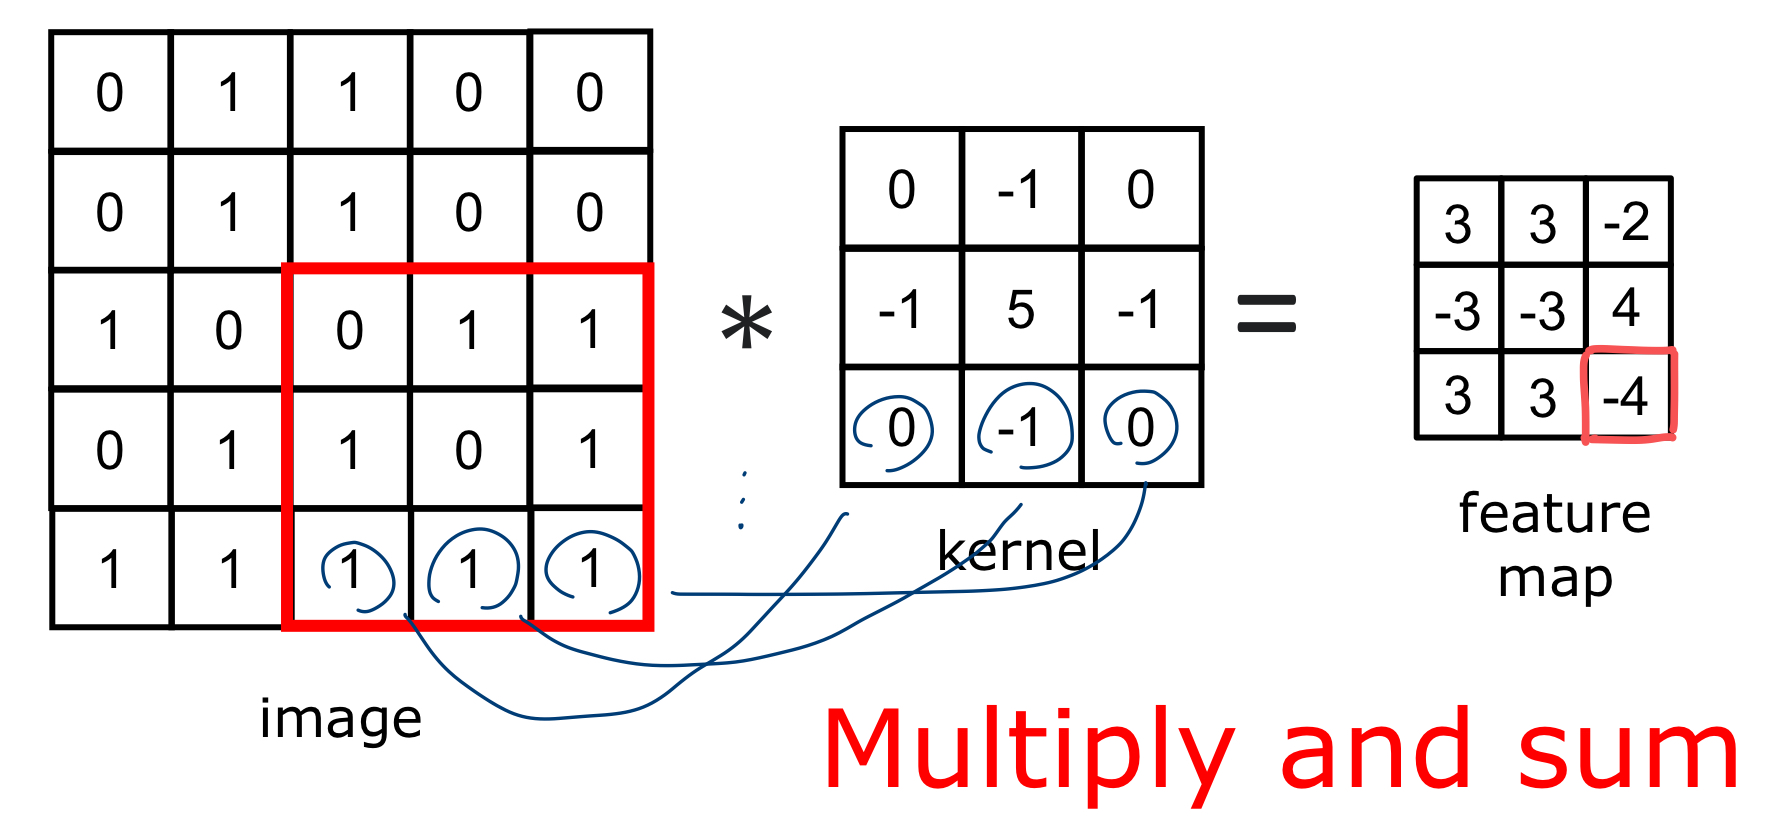
\includegraphics[scale=0.1]{cnn-kernel}

\begin{itemize}
    \item \keyword{Padding}{Add blank pixels at the side to avoid losing edge pixels}
    \item \keyword{Stride}{Skip some pixels by some number of steps for faster computation}
    \item Let $\mathbf{W}^{[l]}$ be kernels, which is a 3D matrix since we apply lots of kernels
\end{itemize}

\[\mathbf{A}^{[l]} = g^{[l]} (\mathbf{W}^{[l]} * \mathbf{A}^{[l - 1]})\]

\begin{itemize}
    \item Each layer has many kernels (3D matrix)
    \item Kernel input: 3D matrix of features maps (Each depth is from diff. kernel)
    \item Kernel output: 2D matrix feature map
    \item \keyword{Pooling}{Reduces dimensionality of feature maps to avoid number of layers exploding (E.g. Max-Pool, Average-Pool, Sum-Pool)}
    \item \keyword{Softmax}{Gets distribution of probabilities to make final classification by taking max. (Similar to multi-class classification)}
\end{itemize}

\[P(y = j) = \frac{e^{x_j}}{\sum_{i = 0}^{k} e^{x_i}}\]

\subsection{Recurrent Neural Network}

\begin{itemize}
    \item Idea: Exploit \textbf{temporal structure} by tracking past values
    \item Not limited to time. As long as there exists a recurring relationship.
    \item Try 1: Have many perceptrons running in parallel for each moment
\end{itemize}

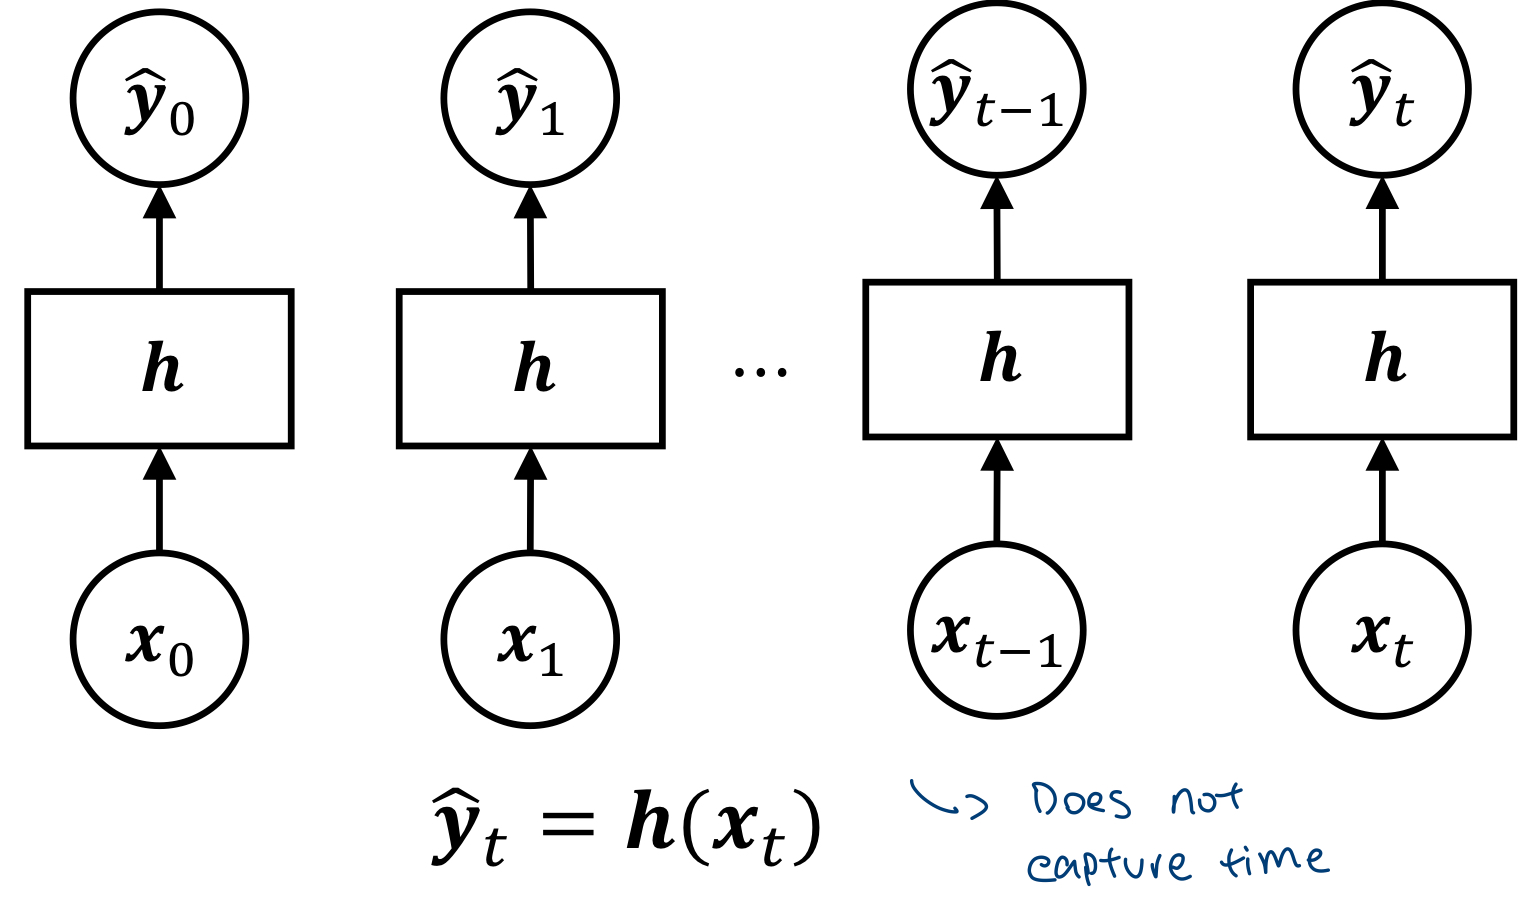
\includegraphics[scale=0.1]{parallel-rnn}

\begin{itemize}
    \item Try 2: Use past perceptron in new one
\end{itemize}

\begin{multicols*}{2}
    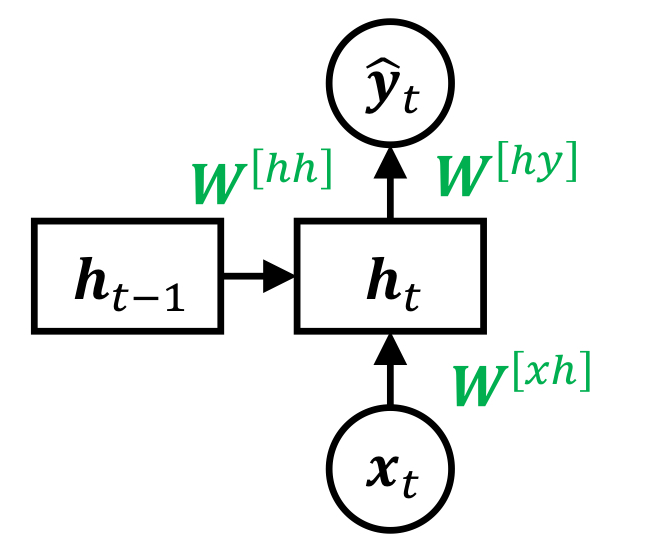
\includegraphics[scale=0.1]{rnn}

    \[\mathbf{y}_t = g^{[y]}((\mathbf{W}^{[hy]})^T \mathbf{h}_t)\]
    \[\mathbf{h}_t = g^{[h]}((\mathbf{W}^{[xh]})^T \mathbf{x}_t +\]
    \[(\mathbf{W}^{[hh]})^T \mathbf{h}_{t-1})\]
\end{multicols*}

\subsection{Problems with Deep Learning}

\subsubsection{1. Overfitting}

\begin{itemize}
    \item \keyword{Drop out}{Randomly set some activations to 0}
    \item \keyword{Early stopping}{Stop training when $J_{test}$ and $J_{train}$ diverge}
\end{itemize}

\subsubsection{2. Vanishing/Exploding Gradient}

\begin{itemize}
    \item \keyword{Vanishing Gradient}{If many gradients $\approx 0$ in backpropagation, then weights won't change}
    \item \keyword{Exploding Gradient}{Gradients keep getting larger, causing GD to diverge}
    \item Solutions:
    \begin{itemize}
        \item Proper weight initialization
        \item Use other activation functions (E.g. ReLU)
        \item Batch normalization (Feature scaling)
        \item Gradient clipping
    \end{itemize}
\end{itemize}

\end{multicols*}
\end{document}
